\documentclass[
    bachelor,
    % bigskip, % sets linespread factor to 1.5
    % nofont, % remember to manally set the fonts
    truefont,
    % sourcefont,
    pdflinks,
    %colorlinks,
    %compact,
    %taskunderline, % 非常 dirty 的方式给任务书中的参考文献加下划线
]{xjtuthesis}

\graphicspath{{figures/}}

%\usepackage{subfigure}

\usepackage{tikz}
\tikzset{add/.style n args={4}{
    minimum width=6mm,
    path picture={
      \draw[black] 
        (path picture bounding box.south east) -- (path picture bounding box.north west)
        (path picture bounding box.south west) -- (path picture bounding box.north east);
      \node at ( $(path picture bounding box.south)+(0,0.13)$ )   {\tiny #1};
      \node at ( $(path picture bounding box.west)+(0.13,0)$ )   {\tiny #2};
      \node at ( $(path picture bounding box.north)+(0,-0.13)$ )    {\tiny #3};
      \node at ( $(path picture bounding box.east)+(-0.13,0)$ )   {\tiny #4};
      }
    }
}
% \usepackage{tikz-er2}
%\usepackage{ulem}
\usepackage{etoolbox}
\usetikzlibrary{positioning}
\input{figures/tikzfig.tex}

\usepackage[simplified]{pgf-umlcd}

\usepackage{pgf-umlsd}

\usetikzlibrary{shapes.geometric,calc,arrows.meta,er,positioning,shapes.geometric}
\usepackage{wrapfig} % 多张图片
\usepackage{overpic} % mask_rcnn
\usepackage{algorithm} % 算法框图
\usepackage{algorithmicx}
\usepackage{algpseudocode}
\usepackage{listings}

\usepackage{color}
\usepackage{xcolor}
\definecolor{dkgreen}{rgb}{0,0.6,0}
\definecolor{gray}{rgb}{0.5,0.5,0.5}
\definecolor{mauve}{rgb}{0.58,0,0.82}
\lstset{frame=tb,
     language=Java,
     aboveskip=3mm,
     belowskip=3mm,
     showstringspaces=false,
     columns=flexible,
     basicstyle = \ttfamily\small,
     numbers=none,
     numberstyle=\tiny\color{gray},
     keywordstyle=\color{blue},
     commentstyle=\color{dkgreen},
     stringstyle=\color{mauve},
     breaklines=true,
     breakatwhitespace=true,
     tabsize=3
}

\floatname{algorithm}{算法}
\renewcommand{\algorithmicrequire}{\textbf{输入:}}
\renewcommand{\algorithmicensure}{\textbf{输出:}}

% \let\cite=\supercite

% 将引用的文献的 BibTeX 放入 bibliography.bib
\addbibresource{bibliography.bib}

\begin{document}

    % 封面信息
    % 标题,中文
\ctitle{基于微信小程序及 SpringBoot 的短视频应用开发}
\covertitlefirst{基于微信小程序及 SpringBoot 的}
\covertitlesecond{短视频应用开发}
\cschool{电气工程}
\cactualinstitution{西安交通大学}
\cmajor{电气工程及其自动化}
\cclass{电气512}
\cyear{\the\year}
\cmonth{\the\month}

% 作者,中文
\cauthor{林子牛}
\stuid{2150400330}

% 学科,中文,本科生不需要
\csubject{}

% 导师姓名,中文
\csupervisor{甘永梅}
    % 任务书信息
    \taskmajor{电气工程及其自动化}
\taskpresident{}
\taskapprovaldate{2019-03-05}
\taskschool{电气工程}
\taskclass{电气~512}
\taskauthor{林子牛}
\tasktitle{基于微信小程序及 SpringBoot 的短视频应用开发}
\taskfromyear{2019}
\taskfrommonth{2}
\taskfromday{26}
\tasktoyear{2019}
\tasktomonth{6}
\tasktoday{1}
\taskplace{西安交通大学}

\taskbackground{
    \uline{SpringBoot 是一个约定大配置的新型 Java Web 框架,其设计目的是简化 Spring 应用开发以及减少不必要的配置。SpringBoot 框架在开发微服务应用方面有着非常大的潜力。}

    \uline{微信小程序是由腾讯开发的新兴的应用分发形式。主要依托于微信,具有开发周期短、应用分发方便以及跨平台等优势。}

    \uline{本毕业设计拟利用 SpringBoot 和微信小程序开发短视频应用程序,其中 SpringBoot 为服务端,微信小程序为客户端。学生在通过此次毕业设计,学习和掌握互联网应用的开发流程、微服务的实践与部署以及了解互联网的体系架构,对于培养学生专业能力以及实践能力非常有帮助。}

%    \uline{超级计算机是计算机中功能最强、运算速度最快、存储容量最大的一类计算机,多用于国家高科技领域和尖端技术研究,是一个国家科研实力的体现,它对国家安全,经济和社会发展具有举足轻重的意义。目前由于成本问题,基于超算的深度学习架构还不够流行,这既限制了科研理论的发展,又没有使超算发挥其应有的作用。}
%
%    \uline{因此,本项目将探索在多CPU集群上的深度行人重识别问题,致力于在项目过程中发现和解决问题,推动理论的发展和实际的应用。}
}

\taskrawmaterial{

	\begin{enumerate}
		\item \uline{SpringBoot Reference Guide}
		\item \uline{Bruce Eckel著,Java 编程思想(第4版),北京:机械工业出版社,2007年}
	\end{enumerate}


%    \uline{在行人重识别领域公认的用于评定一个模型效果的数据集有:VIPeR~\mbox{\cite{gray2007evaluating}}、CUHK01~\mbox{\cite{li2012human}}、CUHK03~\mbox{\cite{li2012human}}、Market-1501~\mbox{\cite{zheng2015scalable}}、DukeMTMC-reID~\mbox{\cite{ristani2016MTMC}}。}
%
%    \uline{毕业设计的资料包括国际上前沿的计算机视觉领域,特别是有关行人重识别问题的期刊、会议论文。~\mbox{\cite{ren2015faster,li2014deepreid,ristani2016MTMC,sun2017beyond,he2017mask,he2016deep,chen2018person}}}
}

\taskmaintask{
	\uline{本毕业设计主要是学习和开发基于SpringBoot的短视频应用。                            
该学生具体的工作内容包括:}
    \begin{enumerate}
        \item \uline{了解和学习微信小程序以及SpringBoot框架的特点及相关技术。}
        \item \uline{采用微信小程序开发应用客户端并上线运行。}
        \item \uline{采用SpringBoot作为服务端框架,使用FFmpeg处理短视频,开发一个短视频应用服务端程序。}
        \item \uline{进一步完成应用调试和测试,验证应用可以可靠地工作。}
        \item \uline{撰写论文并完成约3000字翻译。}
    \end{enumerate}
}

\taskrequirement{
    \begin{enumerate}
        \item \uline{设计的软件功能完备,能够正常在智能手机中运行。}
        \item \uline{论文条理清晰,表述清楚,格式规范。}
        \item \uline{英文翻译正确。}
    \end{enumerate}
}

\taskfinalmaterial{
	\begin{enumerate}
		\item \uline{毕业设计论文一本(A4纸, 1.5万字以上)}
		\item \uline{英文翻译(原文和译文,译文翻译字数在3000字以上)}
		\item \uline{程序源码}
	\end{enumerate}
}

\taskothertaskreference{
	\begin{enumerate}
		\item \uline{Craig Walls著,Spring in Action(Fourth Edition),北京,人民邮电出版社,2016年}
		\item \uline{李华兴等著,Java Web 开发实战经典,北京:清华大学出版社,2010年8月}
	\end{enumerate}
}

\taskteachername{甘永梅}
\taskteacherdate{2019-01-07}
\taskauthorname{}
    % 评审意见信息
    %\input{pages/ch00.2-review}
    % 摘要信息
    % 关键词,中文。用全角分号「;」分割
% 研究生的应首先从《汉语主题词表》中摘选
\ckeywords{Java;短视频应用;数据库优化;视频编码}

% 提交日期,本科生不需要
\cproddate{\the\year 年\the\month 月}

% 论文类型,中文,本科生不需要
% 从理论研究、应用基础、应用研究、研究报告、软件开发、设计报告、案例分析、调研报告、其它中选择
\ctype{}

% 论文标题,英文
\etitle{Short Video Application Development Based on SpringBoot and Wechat Application}

% 作者姓名,英文
\eauthor{Ziniu Lin}

% 学科,英文,本科生不需要
\esubject{}

% 导师姓名,英文
\esupervisor{Yongmei Gan}

% 关键词,英文。用半角分号和一个半角空格「; 」分割
\ekeywords{Java; Short Video Application; Database Optimization; Video Coding}

% 学科门类,英文
% 从Philosophy(哲学)、Economics(经济学)、Law(法学)、Education(教育学)、Arts(文学)、
%   Science(理学)、Engineering Science(工学)、Medicine(医学)、Management Science(管理学)中选择
\ecate{Engineering Science}

% 提交日期,英文,本科生不需要
% 应当和 cproddate 保持一致
\eproddate{\monthname{\month}\ \the\year}

% 论文类型,英文,本科生不需要
% 从Theoretical Research(理论研究)、Application Fundamentals(应用基础)、Applied Research(应用研究)、
%   Research Report(研究报告)、Software Development(软件开发)、Design Report(设计报告)、
%   Case Study(案例分析)、Investigation Report(调研报告)、其它(Other)中选择
\etype{}

% 摘要,中文。段间空行
\cabstract{
	随着无线通讯技术以及智能手机技术的发展,短视频应用获得了巨大的用户基数。短视频应用中比较重要的问题是如何保存大量的用户数据以及如何适当的处理用户上传的大量视频等。如何保存大量用户的数据的问题需要通过合理选择数据库架构、数据库模式以及一定的数据库优化解决。如何适当处理用户上传视频的问题需要通过设置合理地上传方式、视频压制方式以及合理地储存架构来解决。本文通过探寻短视频应用系统开发过程中的各个问题,找出了一些解决方案,这对于解决实际的工程问题以及探寻短视频应用的商业模式有着实际的作用。
	
	本文实现了数据库优化领域的成熟成果,实现了对于数据库系统两方面的优化。第一方面优化为参数优化,在基准测试的衡量下对数据库做整体的优化。第二方面为具体查询优化,针对某一应用、某一查询单独优化数据库系统。这些优化措施在数据库运行时取得了理想的结果。
	
	本文也对视频编码器以及视频压制中的硬件加速效果进行了验证。短视频系统的瓶颈之一就是视频编码器编码速度的问题。通过选用适合短视频应用场景的视频编码器以及使用硬件加速技术可以使得视频压制的过程尽快进行。本文主要通过硬件加速对编码过程进行优化,并且这些优化措施达到了预期目的。

}

% 摘要,英文。段间空行
\eabstract{
    With the development of wireless communication and smart phone, some short video application gains a lot of users. Some serious problems in the development of short video application are how can system store users' information properly and how can system handle the videos provided by users quickly and so on.The first question can be solved by choosing suitable database system structure and the optimization of the database. The second question can be solved by setting suitable upload method, proper video coding algorithm and using right storage method. This paper focus on these problems and get some solution of these problems. This paper will helpful to the solving of really problems and tracking the commercial mode of short video application.
    
    This paper implemented some mature achievements in database optimization and realized two aspects of database system optimization. The first aspect is attribute optimization, which is optimize the whole database under benchmarking. The second aspect is optimizing the database system independently for an application or query. These optimization work very well when the database was running.
    
    This paper also checked the codec and the hardware acceleration effect of video encoding and video compression. One of the bottlenecks of short video system is the encoding speed of video encoder. Through choosing proper video encoder and using hardware acceleration can make doing video compression quickly. This paper mainly optimizes the encoding process through hardware acceleration, and these optimization measures achieve the desired purpose.
}


    % 封面
    \xjtuchead
    % 任务书
    \ctaskdescription
    % 评审意见
    %\creviewopinion
    % 答辩结果
    %\cfinalresult
    % 中文摘要
    \xjtucinfopage
    % 英文摘要
    \xjtueinfopage
    % 目录
    \xjtutoc

    % 主要符号表,可以没有
    %\input{pages/ch00.4-denotation}

    % 正文
    \xjtucontent
    \newrefsection
        % 绪论
        \chapter{绪论}\label{sec:introduction}

本章阐述了此次毕业设计的背景,目前行业内的研究现状,此次毕业设计的研究问题以及此设计的主要工作与创新点等内容。

\section{研究背景}

近年来 随着诸如 4G、高速宽带网络以及智能手机技术的飞速进步。人们的休闲娱乐重心逐渐从文字与图片相关内容转移到了短视频与直播应用上。市场上也涌现出了一系列的短视频应用软件。本毕业设计课题将完成短视频应用开发的整个流程。

目前短视频应用已经成为互联网产业链中一个重要的流量入口。截止 2018 年 12 月,在线视频行业月独立设备数达 10.17 亿,同比增长 1.7\%,其中短视频行业月独立设备数达 7.34 亿台,同比增长率为 58.7\%,用户短视频应用使用时长达到了总上网时长的 8.2\%\cite{中国互联网络信息中心2018第}。在智能手机已经普及的今天,短视频相关应用已经爆发出了强大的活力,具有相当高的市场价值。所以进行短视频应用开发对于我们认识短视频应用相关技术以及商业模式具有非常大的帮助作用。

短视频应用主要功能为接受用户上传的视频并对其进行一系列的处理,如:转码、压缩、合并背景音乐以及提取关键帧等操作。服务器在进行视频相关操作时所承受的压力较大,对于多用户同时上传视频的情景需要设计出一种合理的视频操作解决方案并进行一系列优化。如何合理地处理此种情景也是十分重要的。此外,视频的长度、清晰度、码率、上传的格式也会对服务器的视频操作压力产生影响,因此,本次毕业设计需在视频上传前对视频进行预处理。

当网络应用的用户数较大、同时访问人数较多时,应用系统的瓶颈通常位于服务器的 I/O 输入输出、数据库的操作以及服务器的带宽上,此时,单纯的增加服务器的数量往往不能有效地解决问题\cite{rosenfeld2002information}。因此,合理设计应用系统架构、合理地进行技术选型是非常有用的,有必要对各类型应用架构进行深入地调查、分析与研究。

\section{研究现状}
本节引入了与本设计紧密相关的部分内容:Java Web 技术、数据库技术、视频编码技术以及微信小程序技术。

\subsection{Java Web 技术}

Java Web 技术即使用 Java 语言开发运行在 JVM(Java 虚拟机) 上的网络应用程序的技术。其主要任务是开发出具有合理、高效、低耦合、高内聚、较少错误和较好的可扩展性等优点的应用\cite{arnold2005java}。Java Web 开发需基于 Java 官方给出的 Java EE 规范,且网络应用需运行在 Java 容器或 Java 网络服务器中。随着网络技术以及网络应用的发展,Sun 公司研发了 Servlet 技术。Servlet 是一个能够处理 HTTP 请求的 Java 程序。随着 Servlet 的几轮技术迭代,Sun 公司发布了基于 Java 2 平台的 Java 企业版。由此揭开了 Java 用于网络应用开发的大幕。现在,行业内一般使用某种 Java Web 框架作为基础进行开发,搭配 MVC 技术、ORM 技术以及 Web 服务器进行相关功能的实现。常用的框架有 EJB 框架以及 Spring 框架\cite{williams2014professional}。

EJB 即 Enterprise Java Bean 是一个企业级的 Java 框架,内置了 JBOSS 服务器。图\ref{fig:ejb} 是 EJB 框架的架构图,EJB 框架提供了分布式应用功能,即你可以将一个应用分散到多个服务器上,由多个 Java 虚拟机一同运行\cite{johnson2004expert}。此外 EJB 还提供了组件化支持与持久化管理功能。EJB 技术可以有效地提高 Java 企业级应用开发的效率,但与此同时,EJB 也产生了许多负面影响,如:EJB 使得应用系统更难测试、使应用系统更难部署、破坏了面向对象准则等。因此需要合理地抉择是否使用 EJB。需要使用 EJB 的情景有:应用的部分组件需要被远程访问的情景以及需要对应用进行分布式部署的情景。


% \begin{tikzpicture}
%     % [L1Node/.style={circle,   draw=blue!50, fill=blue!20, very thick, minimum size=10mm},
%     % L2Node/.style={rectangle,draw=green!50,fill=green!20,very thick, minimum size=10mm}]
%     [
%         L1Node/.style={rectangle,draw=green!50,fill=green!20,very thick, minimum size=10mm},
%         Tag/.style={rectangle}
%     ]

%     \draw (0,0) rectangle (10, 15);
%     \node[Tag] (tag1) at (5, 15){EJB 架构图};
%     \node[L1Node] (n1) at (2, 2){JSP};

% \end{tikzpicture}

\begin{figure}[!ht]
    \centering
    %\includegraphics[width=0.7\textwidth]{EJB.png}
    \begin{tikzpicture}
        [
        L1Node/.style={rectangle,draw=green!50,fill=green!20,very thick, minimum width=30mm, minimum height=10mm},
            Tag/.style={rectangle},
			L2Node/.style={rectangle,draw=blue!50,fill=blue!20,very thick, minimum width=30mm, minimum height=10mm},
			L3Node/.style={rectangle,draw=red!50,fill=red!20,very thick, minimum width=30mm, minimum height=10mm},
			L4Node/.style={rectangle,draw=gray!50,fill=gray!20,very thick, minimum width=30mm, minimum height=10mm},
			L5Node/.style={rectangle,draw=purple!50,fill=purple!20,very thick, minimum width=30mm, minimum height=10mm},
        ]
    
        \draw (0.5,0) rectangle (11, 8);
		\draw (1,1.5) rectangle (5, 7);
        \node[Tag] (tag1) at (5.5, 7.5){EJB 架构图};
		\node[Tag] (tag2) at (3, 6.5){EJB 客户端};
        \node[L1Node] (n1) at (3, 5.5){JSP};

\node[L2Node] (n2) at (3, 4){Servlet};
\node[L3Node] (n3) at (3, 2.5){Java App};


\draw (6.5, 0.5) rectangle (10.5, 7);
\node[Tag] (tag3) at (8.5, 6.5){EJB 服务器};
\draw (6.5, 0.5) rectangle (10.5, 6);
\node[Tag] (tag4) at (8.5, 5.5){EJB 容器};
\node[L4Node] (n4) at (8.5, 4.5){Enterprise Bean};
\node[L4Node] (n5) at (8.5, 3){Enterprise Bean};
\node[L5Node] (n6) at (8.5, 1.5){JPA};

\node (n7) at (5,4.25) {};
\node (n8) at (6.5,4.25){};

\draw [->,thick] (n7) to (n8);
\node[Tag] (taga) at (5.75, 4.5){调用};
    
    \end{tikzpicture}
    \caption{EJB 框架架构图}
    \label{fig:ejb}
\end{figure}

Spring 框架是目前非常流行的 Java 框架,图\ref{fig:spring} 展示了 Spring 框架的各模块的组织情况。Spring 框架诞生之初就是为了取代类似 EJB 的重量级 Java 框架。Spring 框架通过扩展 POJO(Plain Old Java Object) 提供了一种轻量、方便的编程方式。Spring 框架提供了依赖注入与面向切面编程帮助用户创建低耦合、高内聚以及高可扩展性的应用程序。Spring 框架非常的灵活,用户可以自由选择应用中每一个模块的功能实现,同时也向用户提供了多种看问题的思路\cite{walls2005spring}。Spring 框架的使用场景非常多,无论是传统网络应用开发还是新兴的微服务系统开发都可以使用 Spring 框架。

\begin{figure}[!ht]
    \centering
    %\includegraphics[width=0.7\textwidth]{spring.png}
    \begin{tikzpicture}
[L1Node/.style={rectangle,draw=green!50,fill=green!20,very thick, minimum width=20mm, minimum height=10mm},
Tag/.style={rectangle},
L2Node/.style={rectangle,draw=blue!50,fill=blue!20,very thick, minimum width=25mm, minimum height=10mm},
L3Node/.style={rectangle,draw=red!50,fill=red!20,very thick, minimum width=20mm, minimum height=8mm},
L4Node/.style={rectangle,draw=gray!50,fill=gray!20,very thick, minimum width=20mm, minimum height=8mm},
GrayNode/.style={rectangle,draw=gray!50,fill=gray!20,very thick, minimum width=45mm, minimum height=8mm},
L5Node/.style={rectangle,draw=purple!50,fill=purple!20,very thick, minimum width=20mm, minimum height=10mm},
BlueBig/.style={rectangle,draw=blue!60,fill=blue!30,very thick,minimum width=112.5mm, minimum height=10mm},
White/.style={rectangle,draw=black!50,fill=white,very thick, minimum width=25mm, minimum height=10mm}]


% 外框
\draw (0.25,0) rectangle (12, 10);
\node[Tag] (t1) at (6.125, 9.5) {Spring 5};

%测试
\node[BlueBig] (n1) at (6.125, 0.75) {测试};

%核心容器
\draw (0.5, 1.5) rectangle (11.75, 3.5);
\node[Tag] (t1) at (6.125, 3.25) {核心容器};
\node[White] (n2) at (2, 2.25) {Beans};
\node[White] (n3) at (4.75, 2.25) {Core};
\node[White] (n4) at (7.5, 2.25) {Context};
\node[White] (n5) at (10.25, 2.25) {Expression};

% 中间部分
\node[L2Node] (n6) at (2, 4.25) {AOP};
\node[L2Node] (n7) at (4.75, 4.25) {Aspects};
\node[L2Node] (n8) at (7.5, 4.25) {Instrument};
\node[L2Node] (n9) at (10.25, 4.25) {Messaging};

% 数据存取
\draw (0.5, 5) rectangle (6, 9);
\node[Tag] (t2) at (3.25, 8.5) {数据存取};
\node[GrayNode] (n10) at (3.25, 5.65) {事务};
\node[L4Node] (n11) at (2, 6.65) {OXM};
\node[L4Node] (n12) at (4.5, 6.65) {JMS};
\node[L4Node] (n13) at (2, 7.65) {JDBC};
\node[L4Node] (n14) at (4.5, 7.65) {ORM};

% Web
\draw (6.25, 5) rectangle (11.75, 9);
\node[Tag] (t2) at (9, 8.5) {Web};
\node[L1Node] (n15) at (7.75, 5.75) {Web};
\node[L1Node] (n16) at (10.25, 5.75) {WebFlux};
\node[L1Node] (n17) at (7.75, 7.25) {WebSocket};
\node[L1Node] (n18) at (10.25, 7.25) {WebMVC};

\end{tikzpicture}

    \caption{Spring 模块组织图}
    \label{fig:spring}
\end{figure}

根据目前互联网业界的经验以及本次毕业设计的需求来看,EJB 框架过于臃肿复杂,不适合本次应用的开发。本次应用开发将使用 Spring 框架,在开发过程中会进行一些迭代,每一次功能增加都会发生在这个时候。Spring 框架的开放性、轻量性与灵活性高度适合互联网应用的开发。因此本次应用设计将基于 Spring 框架进行\cite{walls2016spring}。

在软件开发中的增量模型后,经过几次迭代每个迭代软件开发的一些新的特点,是

\subsection{数据库技术}

数据库是指长期储存在计算机系统内部的、有组织的、可共享的大量数据的集合,数据库中数据按一定数据模型储存,具有有组织、可共享、冗余度低、独立性高以及可扩展性强等特点\cite{王珊2006数据库系统概论}。数据库系统使用数据模型来对数据进行抽象、组织与管理。数据模型可以分为用于设计数据库实际上与任何数据库系统都没有直接关系的概念数据模型和用于具体数据库系统的逻辑与物理数据模型。其中,逻辑数据模型根据使用数据结构的不同还可以分为:层次模型、网状模型、关系模型、面向对象数据模型、对象关系模型以及半结构化数据模型。关系数据模型\cite{bachman1972evolution} 通常被选择为现代数据库系统所使用的逻辑模型。

1970 年 E.F.Codd 提出了关系数据模型。关系数据模型通常具有相对严格的数学模型,每一个关系都像一张记载数据的数据表。关系模型具有许多优点:关系模型的概念比较单一,无论是数据库中抽象出的实体还是这些实体之间的关系都可以用关系表来抽象表示\cite{codd1970relational}。此外,关系模型中的数据操作是集合操作,用户在操作时只需指定做什么而不需要告知数据库怎么做,它的存取路径相对透明,对此极大地方便了用户使用数据库。

随着互联网的发展,关系型数据库逐渐暴露出了诸多弊端:如关系数据库无法有效地处理大量数据的写入、数据更新时改变表的结构以及简单查询迅速返回结果。为了解决这些弊端,开发者们提出了非关系型数据库。非关系型数据库只用于特定领域,几乎不做复杂运算,它具有易于分散数据、方便提升性能的优点。非关系型数据库根据储存原理的不同又可分为:键值型数据库、文档型数据库和列储存数据库等\cite{strauch2011nosql}。键值型数据库原理类似哈希表,一键值对为单元存取数据,其存取速度较快,但存取方式单一,Redis 为键值型数据库最流行的实现。文档型数据库类似一个 JSON 文件,即使不定义表的结构也可像定义了表结构那样使用。MongoDB 是文档型数据库最常用的实现。

\subsection{视频编码技术}

视频编码技术是对视频进行压缩以更好地适应网络传输的技术。目前最新的视频编码国际标准 - 高效视频编码HEVC,已于2013年由JCT-VC正式颁布,其压缩性能在前一代H.264/AVC的基础上提高了一倍。优秀的视频编码可以有效地在尽可能小地影响画质的基础上对视频进行大幅度地压缩\cite{万帅2014新一代高效视频编码}。视频编码技术在本设计中有着重要的作用。

\subsection{微信小程序}
微信小程序是一种基于微信的混合应用。微信小程序使用方便、无需安装、不占空间、用完即走。本程序用户交互端基于微信小程序。

\section{论文的主要工作}

本节介绍了本次毕业设计中的各项具体工作。

首先,本文详细阐述了此次毕业设计使用的各种技术的原理以及整个短视频应用系统架构的设计。在应用系统开发完成后在云服务器平台进行部署与测试。

随后,本文试验了各种数据库优化的方法并对它们进行比较,找出了最适合本系统的数据库解决方案,并与初始状态进行了比较。

最后,本文提出了比较适合短视频应用场景的视频压缩编码方案,对于短视频这种视频长度较小、主要基于移动端以及对画质要求低流畅度要求高等特性做出了对应的优化措施,提高了视频编码时的性能表现。




\section{论文的组织结构}

本文主要结构如下:第~~\ref{sec:theory}~~章讲述了本文主要使用的技术框架与理论。第~~\ref{sec:algorithm}~~章详细讲述了项目各部分的具体实现优化措施。第~~\ref{sec:experiment}~~章展示项目开发成果与优化结果。第~~\ref{sec:conclusion}~~章总结了项目和论文。

        % 理论框架
        \chapter{设计原理}\label{sec:theory}

\section{Spring 框架}

近年来 Spring 框架是 Java Web 框架中经常被使用的,其主要目的是降低应用系统开发时的复杂性。Spring 框架构建基于其核心,Spring 核心模块提供了一个 IoC 容器以及一些举出工具类。Spring AOP 模块位于核心模块之上,这为开发者提供了一系列面向切面编程支持。在 AOP 模块之上是数据访问与事务管理功能\cite{walls2005spring}。下文将详细介绍这三个 Spring 框架的基础功能。

\subsection{Spring 框架的控制反转容器}

控制反转 (Inversion of Control, IoC) 概念来源于依赖倒置原则。依赖倒置原则即高层模块不应该依赖低层模块,二者都应该依赖其抽象;抽象不应该依赖细节;细节应该依赖抽象\cite{gamma1995design}。简单地说,高层模块与低层模块不应该直接产生耦合,高层与低层模块应通过一个接口耦合在一起,即高层模块依赖于该接口,低层模块实现该接口。如图 \ref{fig:beforeAndAfter} 所示,这样对于低层模块的修改就不会对高层模块产生较大的影响同时也减小了系统各模块的耦合。

\begin{figure}[!ht]
\centering
\subfloat[使用 IoC 前]{
	\centering
    %\includegraphics[width=0.5\textwidth]{beIOC.png}}
    \begin{tikzpicture}
        \begin{class}{高层模块}{0,0}
            \attribute{低层模块 : 依赖}
            \operation{高层模块方法 : 返回值}
            % virtual operation
            \end{class}
            
            \begin{class}{低层模块}{7.5,0}
            \attribute{属性}
            \operation{方法}
            % virtual operation
            \end{class}
            
            \aggregation{高层模块}{}{依赖}{低层模块}
    \end{tikzpicture}}\quad
\subfloat[使用 IoC 后]{
    \centering
    %\includegraphics[width=0.5\textwidth]{afIOC.png}
    \begin{tikzpicture}
\begin{interface}{低层模块接口}{0,0}
    \attribute{接口属性}
    \attribute{接口方法} \end{interface}
    
    \begin{class}{高层模块}{-3,-3}
    \attribute{低层模块 : 依赖}
    \operation{高层模块方法 : 返回值}
    % virtual operation
    \end{class}
    
    \begin{class}{低层模块}{3,-3}
    \implement{低层模块接口}
    \attribute{底层模块属性}
    \operation{低层模块方法}
    % virtual operation
    \end{class}
    
    \aggregation{高层模块}{}{依赖}{低层模块接口}
    \end{tikzpicture}
    }
\caption{使用 IoC 前后 UML 图}
\label{fig:beforeAndAfter}
\end{figure}

Spring 的控制反转容器是通过依赖注入 (Dependency Injection, DI) 实现的。如图 \ref{fig:DI} 所示,依赖注入即高层模块在使用低层依赖时,不是自己将低层模块实例化而是向控制反转容器申请一个已创建好的依赖对象\cite{prasanna2009dependency}。这样高层模块与低层模块间的耦合被降低了,对于低层模块的改变对高层模块产生的影响也变小了。同时,由于低层模块由容器创建,我们就可以轻松地实现单例模式等设计模式,进一步简化了开发也提高了系统的性能。通过使用 Spring 框架提供的 IoC 容器,我们可以轻松地使用控制反转构建应用系统。

\begin{figure}[!ht]
    \centering
    \includegraphics[width=0.6\textwidth]{IoC.png}
    \caption{Spring 依赖注入作用}
    \label{fig:DI}
\end{figure}

\subsection{Spring AOP 框架}

在一个应用系统中存在着一些许多模块公用的功能,如:日志记录、安全检查以及事务功能等。这些公用功能如果处置不当就会造成系统的代码冗余度增加和耦合性上升,例如:要在系统中增加一次日志记录,我们就必须在所有的模块中加入相同的代码,着无疑是非常低效的。对此,我们可以使用面向切面编程 (Aspect Oriented Programming) 来解决这一问题。


\begin{figure}[!ht]
    \centering
    %\includegraphics[width=0.4\textwidth]{AOP.png}
    \begin{tikzpicture}
        [Tag/.style={rectangle}]
        \draw (0,0) rectangle (8, 1);
        \draw (0,-1.5) rectangle (8, -0.5);
        \draw (0,-3) rectangle (8, -2);
        \node[anchor=center] (n1) at (3, -1){\includegraphics[scale=0.6]{arrow}};
        \node[anchor=center] (n2) at (5, -1){\includegraphics[scale=0.6]{arrow}};
        \node[anchor=center] (n3) at (7, -1){\includegraphics[scale=0.6]{arrow}};
        \node[Tag] (t1) at (0.6, 0.5) {服务 A};
        \node[Tag] (t2) at (0.6, -1) {服务 B};
        \node[Tag] (t3) at (0.6, -2.5) {服务 C};

        \node[Tag] (t4) at (3, 2.25) {日志};
        \node[Tag] (t5) at (5, 2.25) {安全};
        \node[Tag] (t6) at (7, 2.25) {事务};

    \end{tikzpicture}
    \caption{面向切面编程中的横切关注点}
    \label{fig:AOP}
\end{figure}

如图 \ref{fig:AOP} 所示,面向切面编程可以将系统中的公共功能抽象成为许多称之为横切关注点的功能模块,例如:日志记录功能就是一个横切关注点。系统中需要使用这些公共功能的地方称之为连接点 (Joinpoint)\cite{walls2005spring}。在系统运行时面向切面编程框架会将横切关注点织入连接点中,这样系统就可以使用所有的公共功能,减少了系统的冗余代码与耦合性。

Spring 框架中的面向切面编程功能由动态代理实现,源于设计模式中的代理模式。如图 \ref{fig:Proxy} 所示,代理模式的作用是为隔离被代理对象,使用代理提供功能调用\cite{gamma1995design}。代理处于访问者与被访问者之间,隔离两者的直接交互。在代理将访问者的访问请求传递给被访问者时,代理可以添加一部分额外的功能,如安全检测。因此,代理模式可以有效地增强系统的灵活性与安全性。动态代理的实现还要依靠 Java 提供的反射功能。反射功能允许我们在 Java 程序的运行期间动态载入类、创建对象以及生成代理。通过实现代理模式、使用反射机制,我们就可以创建出动态代理系统,实现面向接口编程\cite{walls2005spring,walls2016spring}。

\begin{figure}[!ht]
    \centering
    %\includegraphics[width=0.6\textwidth]{Proxy.png}
    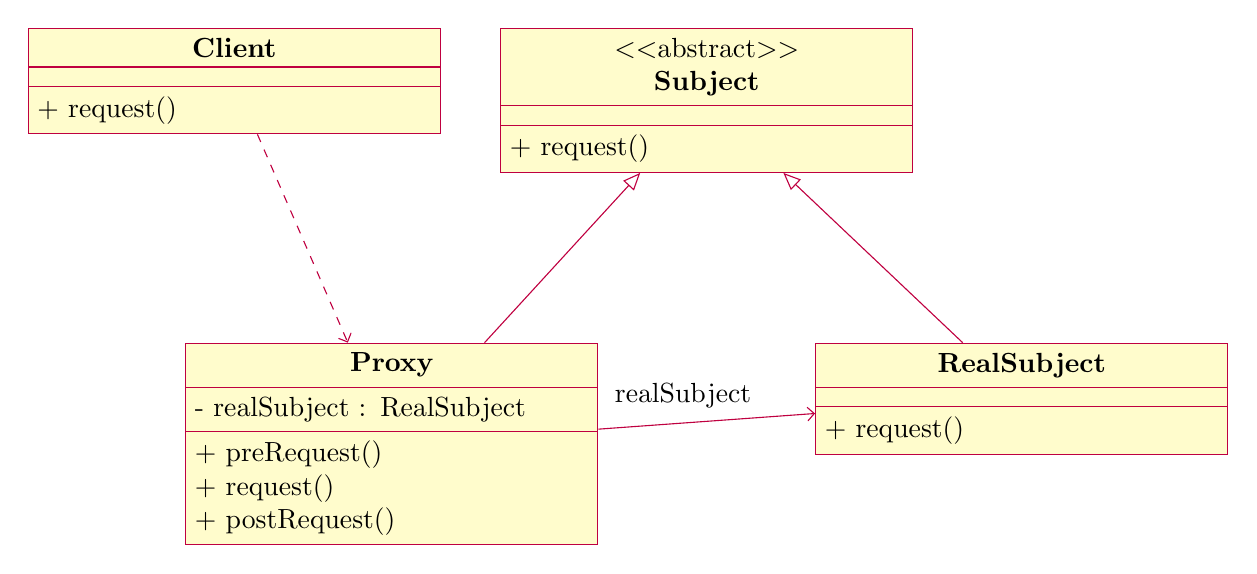
\begin{tikzpicture}
\begin{abstractclass}{Subject}{0 ,1}
    \attribute{}
    \operation{+ request()}
    \end{abstractclass}
    
    \begin{class}{Proxy}{-4,-3}
    \inherit{Subject}
    \attribute{- realSubject : RealSubject}
    \operation{+ preRequest()}
    \operation{+ request()}
    \operation{+ postRequest()}
    % virtual operation
    \end{class}
    
    \begin{class}{RealSubject}{4,-3}
    \inherit{Subject}
    \attribute{}
    \operation{+ request()}
    % virtual operation
    \end{class}
    
    \begin{class}{Client}{-6,1}
    \attribute{}
    \operation{+ request()}
    % virtual operation
    \end{class}
    
    \unidirectionalAssociation{Proxy}{realSubject}{}{RealSubject}
    
    \draw[umlcd style dashed line, ->] (Client) --node[above, sloped, black]{} (Proxy);
    
    \end{tikzpicture}
    \caption{代理模式 UML 图}
    \label{fig:Proxy}
\end{figure}

Spring AOP 的设计遵循了 8/2 原则,即通过 20\% 的代码实现 AOP
 框架 80\% 的功能。因此Spring AOP 支持的 AOP 功能是不完全的,例如 Spring AOP 不支持属性级别的拦截等。系统运行时,我们在系统中定义所有的切面、连接点都会被 Spring AOP 拼装起来,这个操作被称为织入\cite{spring2019}。织入时,Spring 会自动生成切面的代理包装类,通过代理包装类将切面织入代码中。Spring AOP 框架为我们提供了 AOP 的大部分功能,同时我们也可以整合使用 AspectJ 等框架来获取 Spring AOP 不支持的功能。
 
 \subsection{Spring 事务管理功能}
 
 事务管理的作用是保证应用系统在操作数据库时不会对数据的正确性产生破坏,具体的事务定义将在下文介绍。在 Spring 框架中,我们通常使用声明式的方式使用事务,事务也是一个常用的 AOP 中的横切关注点。通常情况下使用事务,我们需在每次访问数据库前声明事务开始,在事务正常结束后进行结束事务操作,在事务异常结束后进行事务的回滚。Spring 框架使用 AOP 来处理事务,通过在运行时将事务代码织入应用中来简化开发\cite{spring2019,walls2005spring}。
 
 我们在需要使用事务的地方使用 @Transactional\cite{spring2019} 注解即可开启声明式事务功能。我们可以在其中设置一些事物属性。事务属性主要包括:隔离级别、传播行为、回滚规则、是否只读以及超时时间等。通过注解使用声明式事务对于简化数据访问层的开发具有较大的意义\cite{walls2016spring}。


\section{数据库的原理与设计}

本次设计采用 MySQL 作为系统主数据库、Redis 作为缓存数据库。


\subsection{关系型数据库}
支持关系模型的数据库系统为关系型数据库系统。关系模型主要数据结构为关系{codd1970relational}。关系中的域是一组具有相同数据类型的值的集合。一个关系可以由多个域的笛卡尔积表示。如一个班中所有学生的年龄的集合就是一个域\cite{王珊2006数据库系统概论}。

笛卡尔积是一种域上的集合运算,其定义为:
\begin{equation}
\label{eq:Descartes}
D_1 \times D_2 \times \cdots \times D_n = {(d_1, d_2, \cdots, d_n) | d_i \in D_i, i=1, 2, \cdots, n}
\end{equation}
其中,每一个元素 $(d_1, d_2, \cdots, d_n)$ 为一个元组。笛卡尔积可以表示一个二维表,表中的一行对应笛卡尔积中的一个元组。$D_1 \times D_2 \times \cdots \times D_n$ 的子集为在域 $D_1, D_2, \cdots, D_n$ 上的关系\cite{codd1970relational}。

每一个关系中都存在一些特殊的属性。若关系中某一属性组可以唯一标志该元组,而其任意子集均无此性质,则该属性组为这个关系的候选码。任意包含在至少一个候选码中的属性为主属性,不包含在所有候选码中的属性为非主属性。在任意关系表中不可能存在具有相同候选码的两个或多个元组\cite{codd1970relational,王珊2006数据库系统概论}。

关系模式可以表示为 $R(U, D, DOM, F)$,其中 $R$ 为关系名,$U$ 为属性名的集合,$D$ 为域的集合,$DOM$ 为属性与域的映射,$F$ 为属性间的依赖关系。关系模式中主要包含关系中有哪些属性、关系中有哪些域以及域与属性的映射关系。

关系数据模型中具有关系的操作。集合操作有:并 (union, $\cup$ ) 、差 (except, $-$ ) 、交 (intersection, $\cap$ ) 、除 (divide, $\div$ ) 和笛卡尔积 (Descartes Product, $\times$ )。关系专用操作包括:选择 (select, $\sigma$) 、投影 (project, $\Pi$) 以及连接 (join, $\Join $)。其中,选择、投影、并、差、笛卡尔积是基本操作\cite{ullman1984principles}。

\begin{figure}[!ht]
    \centering
    %\includegraphics[width=0.4\textwidth]{db1.png}
    \begin{tikzpicture}
[Tag/.style={rectangle},
Block/.style={rectangle,draw=black,fill=white,very thick, minimum width=65mm, minimum height=10mm},
Block2/.style={rectangle,draw=black,fill=white,very thick, minimum width=20mm, minimum height=20mm}]

\node[cylinder,draw=black,thick,aspect=0.7,minimum height=1.7cm,minimum width=1.5cm,shape border rotate=90,cylinder uses custom fill, cylinder body fill=red!30,cylinder end fill=red!10] (A) at (0,0) {引擎};

\node[cylinder,draw=black,thick,aspect=0.7,minimum height=1.7cm,minimum width=1.5cm,shape border rotate=90,cylinder uses custom fill, cylinder body fill=red!30,cylinder end fill=red!10] (A) at (1.75, 0) {引擎};

\node[cylinder,draw=black,thick,aspect=0.7,minimum height=1.7cm,minimum width=1.5cm,shape border rotate=90,cylinder uses custom fill, cylinder body fill=red!30,cylinder end fill=red!10] (A) at (3.5, 0) {引擎};

\node[cylinder,draw=black,thick,aspect=0.7,minimum height=1.7cm,minimum width=1.5cm,shape border rotate=90,cylinder uses custom fill, cylinder body fill=red!30,cylinder end fill=red!10] (A) at (5.25, 0) {引擎};

\draw (-1,1.2) rectangle (6.2, 7.75);

\node[Block] (b1) at (2.6, 2.25) {优化器};
\node[Block2] (b2) at (1, 4.5) {查询缓存};
\node[Block2] (b3) at (4.2, 4.5) {解析器};

\node[Block] (b4) at (2.6, 6.75) {连接/线程处理器};

\node[Tag] (t1) at (2.6, 8.75) {客户端};

\node[Tag] (t2) at (2.6, 7.65) {};

\draw[-{Stealth[length=3mm, round]}] (4.2,3.5)--(4.2,2.75);
\draw[-{Stealth[length=3mm, round]}] (3.2,4.5)--(2,4.5);
\draw[-{Stealth[length=3mm, round]}] (4.2,6.25)--(4.2,5.5);
\draw[-{Stealth[length=3mm, round]}] (1,6.25)--(1,5.5);
\draw[-{Stealth[length=3mm, round]}] (2.6,8.5)--(2.6,7.75);
    \end{tikzpicture}
    \caption{MySQL 架构分析图}
    \label{fig:db1}
\end{figure}


\subsection{数据库事务}

数据库事务是用户定义的一个数据库操作序列,是不可分割的工作单位。事务具有四个特征,分别是原子性:一个事务是不可分割的,事务内所有操作的状态必须一致;一致性:事务的作用必须使数据库从一个一致状态变为另一个一致状态;隔离性:多个事务的执行互不干扰;持续性:事务对数据库的修改是永久的。数据库事务是在并发条件下保证数据库数据正确的总要条件。

\subsection{MySQL 原理}
MySQL 是一个开源的关系型数据库管理系统。MySQL 非常的灵活,可以适应多种运行场景,例如:MySQL 既可以嵌入在程序中运行也可以支持数据仓库、在线处理系统等应用\cite{姜承尧2011mysql}。MySQL 主要由两部分组成:客户端与服务端。客户端的作用是向数据库系统发出命令并获取命令执行结果。服务端就是数据库系统本身,负责处理查询语句、执行查询并将查询结果返回客户端。

MySQL 是一个层次化系统,如图 \ref{fig:db1} 所示,主要包括 SQL 接口、查询 MySQL 解析器、MySQL 查询优化器以及查询执行引擎、缓冲/缓存机制和一个插件式的储存引擎。第二层服务是 MySQL 的核心,第三层则包括了储存引擎,它负责数据库中数据的储存与提取。我们可以根据需要选择不同功能的查询引擎\cite{schwartz2012high}。


MySQL 默认的库表结构与查询优化是不能有效地满足应用性能需求的,为此,我们需对 MySQL 的运行过程进行合理地优化。为了实现 MySQL 的高性能运行,我们需要对 MySQL 进行查询优化、索引优化以及库表结构优化。库表结构优化指为数据库选取合适的数据类型、合理使用 MySQL 特性以及使用缓存等操作。索引优化指在数据库表中的某些列上添加正确的索引以加快查询速度。查询优化指合理设置查询方式,使得查询产生的中间结果最少、查询过程合理使用索引及物理结构,使得查询速度加快。

\subsection{数据库设计原理}

本项目中采用基于 E-R (Entity - Relation, 实体 - 关系) 模型的设计方法进行设计。如图 \ref{fig:db2} 所示,数据库设计主要分为六个阶段:需求分析、概念设计、逻辑设计、物理设计、数据库实施以及数据库运行与维护\cite{王珊2006数据库系统概论}。

\begin{figure}[!ht]
    \centering
    %\includegraphics[width=0.4\textwidth]{db2.png}
    \begin{tikzpicture}
[Tag/.style={rectangle},
White/.style={rectangle,draw=black,fill=white,very thick, minimum width=65mm, minimum height=10mm},
White2/.style={rectangle,draw=black,fill=white,very thick, minimum width=20mm, minimum height=20mm},]

\node[White] (b1) at (0, 0) {使用/维护数据库};
\node[White] (b2) at (0, 1.75) {试运行};
\node[White] (b3) at (0, 3.5) {物理实现};
\node[White] (b4) at (0, 5.25) {评估设计、预测性能};
\node[White] (b5) at (0, 7) {物理结构设计};
\node[White] (b6) at (0, 8.75) {数据模型优化};
\node[White] (b7) at (0, 10.5) {逻辑结构设计};
\node[White] (b8) at (0, 12.25) {概念结构设计};
\node[White] (b9) at (0, 14) {需求分析};

\draw[-{Stealth[length=3mm, round]}] (b9)--(b8);
\draw[-{Stealth[length=3mm, round]}] (b8)--(b7);
\draw[-{Stealth[length=3mm, round]}] (b7)--(b6);
\draw[-{Stealth[length=3mm, round]}] (b6)--(b5);
\draw[-{Stealth[length=3mm, round]}] (b5)--(b4);
\draw[-{Stealth[length=3mm, round]}] (b4)--(b3);
\draw[-{Stealth[length=3mm, round]}] (b3)--(b2);
\draw[-{Stealth[length=3mm, round]}] (b2)--(b1);

\draw[-{Stealth[length=3mm, round]}] (3.25, 5.25)--(4, 5.25)--(4, 10.5)--(3.25,10.5);

\draw[-{Stealth[length=3mm, round]}] (3.25, 5.25)--(4, 5.25)--(4, 7)--(3.25,7);

\draw[-{Stealth[length=3mm, round]}] (-3.25, 1.75)--(-4, 1.75)--(-4, 7)--(-3.25,7);

\node[Tag] (t1) at (4.75, 5.5) {不满意};
\node[Tag] (t2) at (-5, 2) {不满意};

    \end{tikzpicture}
    \caption{数据库设计流程图}
    \label{fig:db2}
\end{figure}

设计数据库时,首先必须分析设计需求,需求分析过程是整个设计的基础。随后,在需求分析的基础上开始概念结构设计,产出数据库概念结构。完成概念设计后,进行逻辑结构设计,将概念模型转换为数据库管理系统支持的逻辑模型,并进行优化。随后进行物理结构设计,即为设计好的逻辑结构选取最合适的物理结构。物理结构设计完成后,使用数据库语言建立相应的数据库、调试并进行数据入库。完成上述过程后,数据库即可开始运行,在运行时需根据实际情况作出调整与适当地维护\cite{wiederhold1983database}。

\section{微信小程序}

微信小程序的开发要基于微信小程序开发框架。微信小程序开发框架将微信小程序分为逻辑层与视图层。逻辑层由 JavaScript 语言编写,负责处理小程序的逻辑操作与后端交互。视图层由 wxml 和 wxss 编写,负责渲染出开发者想要的页面。微信小程序的开发以页面为单位,每个页面都是一个独立的单位。开发时,首先要在配置文件中注册所有的页面,随后便可以逐个页面进行开发。


\section{视频编码}

在网络上进行传输的视频必须经过编码与压缩。网络传输的高清视频分辨率通常为 1920 $\times$ 1080,帧率为 30 帧,这样的视频如果不进行编码与压缩,一秒钟的视频产生文件大小为 177M 字节,移动网络大部分情况都不能以如此高的速率加载视频。因此要对视频进行编码与压缩,以某种方式压缩视频的算法称为视频编码。

目前主流的视频编码有 h.264\cite{richardson2004h} 和 h.265\cite{万帅2014新一代高效视频编码} 编码。h.264 编码比较成熟与稳定,目前所有的移动设备均能流畅解码播放,兼容性较好同时其编码器效率较高,编码速度较快,同时 h.264 编码的缺陷在于压缩率不如 h.265 编码。h.265 编码是最新的视频编码,h.265 编码的压缩率较高,h.265 编码视频只需使用 h.264 编码视频码率的一般即可达到同样的画质效果。h.265 编码的缺陷在于兼容性不如 h.264 编码,且编解码所需时间较长。

视频编码常用压缩算法主要有帧间压缩和帧内压缩。帧内压缩就是将视频的每一帧图像都进行有损压缩,如 Jpeg 压缩。其基本原理为应用人眼对亮度敏感同时对色彩不敏感的特性,尽可能保留图像的亮度信息,大幅压缩图像的色彩信息,以减小图像的大小。帧间压缩的原理是不保存视频所有的帧,只保留视频的关键帧以及两个关键帧之间像素的变化情况,具体原理如图 \ref{fig:video1} 所示。帧间压缩通常采用帧间预测编码来实现\cite{richardson2004h}。

\begin{figure}[!ht]
    \centering
    %\includegraphics[width=0.6\textwidth]{video1.png}
\begin{tikzpicture}
    [Tag/.style={rectangle},
White/.style={rectangle,draw=black,fill=white,very thick, minimum width=20mm, minimum height=10mm}]

\node[draw,circle,minimum width=0.5cm,add={}{}{}{}] (circle) at (0,0) {};
\node[Tag] (t1) at (-2, 0) {};
\node[Tag] (tn) at (10, 0) {};
\node[Tag] (t2) at (-1, 0.25) {$f_{t}(x,y)$};

\node[Tag] (t3) at (1.5, 0.25) {$e_{t}(x,y)$};

\node[White] (w1) at (4, 0) {量化器};

\node[White] (w2) at (2, -3) {运动补偿预测器};

\node[Tag] (t4) at (-0.6, -1.5) {$\hat{f}_{t}(x,y)$};

\node[White] (w3) at (6, -3) {帧储存器};
\node[draw,circle,minimum width=0.5cm,add={}{}{}{}] (circle2) at (8,-2) {};

\node[Tag] (t5) at (4, -1.7) {$\hat{f}_{t}(x,y)$};

\node[White] (w4) at (2, -5) {运动参数估计器};

\node[Tag] (t5) at (5, -4.5) {前帧或后帧};
\node[Tag] (t6) at (7, 0.25) {$e^{'}_{t}(x,y)$};

\node[Tag] (t6) at (7.3, -4) {$f^{'}_{t}(x,y)$};
\node[Tag] (t6) at (7.3, -5.7) {当前帧};

\draw[-{Stealth[length=3mm, round]}] (t1)--(circle); 
\draw[-{Stealth[length=3mm, round]}] (circle)--(w1); 
\draw[-{Stealth[length=3mm, round]}] (w2)--(0, -3)--(circle); 
\draw[-{Stealth[length=3mm, round]}] (w3)--(w2); 
\draw[-{Stealth[length=3mm, round]}] (w2)--(0.4, -3)--(0.4, -2)--(circle2);
\draw[-{Stealth[length=3mm, round]}] (w4)--(w2);
\draw[-{Stealth[length=3mm, round]}] (w3)--(4,-3)--(4, -5)--(w4);
\draw[-{Stealth[length=3mm, round]}] (w1)--(tn);
\draw[-{Stealth[length=3mm, round]}] (w1)--(8, 0)--(circle2);
\draw[-{Stealth[length=3mm, round]}] (circle2)--(8, -6)--(2, -6)--(w4);
\end{tikzpicture}
    \caption{单向预测帧间编码}
    \label{fig:video1}
\end{figure}

帧间预测编码的基础是单向预测算法。单向预测算法通常将视频整个画面划分为若干块,以块为单位分配运动矢量\cite{毕厚杰2005新一代视频压缩编码标准}。如图 \ref{fig:video1} 所示,把当前帧 $f_{t}^{'})(x,y) $ 与前一帧 $f_{t-1}(x,y)$ 输入运动参数估计器中,运算后得到运动矢量,运动矢量输入补偿器得到预测图像 $\hat{f}_{t}(x,y)$。利用上一帧图像与运动矢量得到当前图像的算法称为单向预测算法:
\begin{equation}
\label{eq:forward_pre}
\hat{f}_{t}(x,y) = f_{t}(x+i, y+i)
\end{equation}
其中,$(i, j)$ 为运动矢量。目前通常采用基于单向预测算法的双向预测算法,即同时利用前一帧图像与后一帧图像进行预测:
\begin{equation}
\label{eq:forward_back_pre}
\hat{f}_{t}(x,y) = \alpha_{t-1}f_{t}(x+i, y+i) + \alpha_{t+1}f_{t}(x+i^{'}, y+i^{'})
\end{equation}
双向预测算法不可用于实时视频当中,只能用于实现录制好播放的视频中。

h.264 编码的视频中主要包含三种类型的帧:I 帧、P 帧以及 B 帧,表示运动补偿形式的不同。其中,I 帧为帧内编码帧也叫关键帧,保留完整的图像信息,对于视频进度条跳转有很大帮助。P 帧为帧间预测编码帧,且只能前向预测,它只参考前面最靠近它的I帧或者P帧。B 帧也是帧间预测编码帧, 它可以双向预测。每一个 I 帧以及它与下一个 I 帧之间所有的 P 帧与 B 帧称为一个 GOP 序列。B 帧的压缩率最大,解码的性能也最差,大量使用 B 帧可以节省空间放入更多的 I 帧,相同码率下画质会更好。因此在编码时要合理地设置 GOP 序列大小以及 B 帧的使用\cite{richardson2004h}。

\subsection{数据库与视频编码优化评价标准}
\subsubsection{数据库优化评价标准}
MySQL 主要测试指标有:吞吐量、响应时间、并发性以及可扩展性。吞吐量是指数据库每秒处理的事务的数量。数据吞吐量对于有大量用户同时访问的应用系统来说十分重要,直接决定系统的承载能力,常用测试单位为每秒事务数 (TPS)。响应时间指数据库系统完成一个任务所需要的平均时间,响应时间过长会造成数据库并发瓶颈,通常使用百分比响应时间 (percentile response time, PRT) 作为单位。并发性指数据库系统允许多少请求同时访问,通常测试并发数增加与吞吐量变化的关系。可扩展性指数据库系统在数据量增大时,能否增强其处理能力的特性\cite{schwartz2012high}。

\subsubsection{视频编码评价标准}

视频编码的评价标准主要有编码后视频的体积、编码时间以及某一码率下视频画质。编码后视频体积表示了当前编码器设置的压缩率好坏。编码所用时间表示编码一段短视频耗费时间,视频编码时间不能过长。视频画质表示码率一定时不同编码方案的画质好坏,采用峰值信噪比 ($PSNR$) 作为单位\cite{毕厚杰2005新一代视频压缩编码标准},计算方法:
\begin{equation}
\label{eq:forward_back_pre}
PSNR_{dB} = \frac{10log_{10}(2^{n} - 1)^{2}}{MSE}
\end{equation}
其中 $MSE$ 为原始视频与编码后视频图像之间的均方误差,n 为每个像素的比特数。

\section{本章小结}
本章讲述了本文主要使用的技术框架与理论,包括 Spring 框架、数据库设计与优化技术以及视频压制优化技术等,这些框架与技术有着重要的作用。下一章将叙述应用系统具体实现方案与对应的优化操作。








        % 算法实现
        \chapter{项目内容及优化实现}\label{sec:algorithm}

本章介绍了项目在准备阶段和项目各部分优化细节。项目的准备阶段包括数据库的设计与实施、系统代码的编写以及短视频压缩编码的初步实现。优化细节包括数据库性能瓶颈分析与消除、数据库语句优化以及视频压制优化。

\section{数据库的设计}
 
\subsection{需求分析}
设计数据库首先要进行需求分析\cite{gamma1995design}。本系统需要数据库来管理与储存用户信息、视频信息、视频的评论信息用户以及用户与视频的各种关系。用户信息包含用户的系统内唯一编号、用户名、密码、注册时间、用户头像以及用户各项统计信息等内容。视频信息包括视频名称、视频文件存放位置、视频作者、视频相关统计信息等内容。评论信息包含评论人、评论内容、评论种类、评论视频等内容。用户与视频关系包含关系类型、用户编号与视频编号等内容。

为了需求分析的简便,我们先将用户与视频所有的信息放入一张表中,其 E-R 图如图 \ref{fig:ER1} 所示。随后我们要进行关系的规范化。

\begin{figure}[!ht]
    \centering
    \includegraphics[width=0.5\textwidth]{dbs1.png}
    \caption{需求分析数据库 E-R 图}
    \label{fig:ER1}
\end{figure}


\subsection{关系规范化}

经过初步地需求分析后,我们得到了一个初步地数据库模型,但这个模型仅仅遵循了关系数据库理论的第一范式\cite{codd1972further},即所有的属性均为原子属性。仅遵循第一范式的模型有插入异常、删除异常以及修改复杂等缺点。以此模型中的用户表为例。当一个用户没有任何视频时无法将该用户插入,导致更新异常。当一个用户信息需变更时需改变所有包含用户信息的元组,导致修改复杂。当用户删除所有视频时会导致用户信息被一同删除,导致删除异常。

为了解决这些问题,我们需要使数据库符合第二范式\cite{codd1972further},即关系遵循第一范式,且关系中所有的非主属性都完全函数依赖于任何候选码。为了使关系遵循第二范式,我们要对其进行规范化,即将一个大的关系拆分为两个或多个小的关系。我们将用户表拆分为用户信息表和视频信息表,两个表的函数依赖关系在拆分后由外健保留,关系拆分后 E-R 图 (省略实体的属性) 如图 \ref{fig:ER2} 所示 。

\begin{figure}[!ht]
    \centering
    \includegraphics[width=0.6\textwidth]{dbs2.png}
    \caption{规范化后数据库 E-R 图}
    \label{fig:ER2}
\end{figure}

经过关系分解后,用户表与视频表中即不存在关于主属性的传递函数依赖,也不存在非主属性决定子,所以分解后整个关系达到了 BCNF\cite{bernstein1976synthesizing},解决了之前可能出现的问题。

\subsection{数据库逻辑结构设计}

完成数据库的概念结构 (E-R 模型) 后开始设计数据库逻辑结构\cite{gamma1995design}。这里我采用将 E-R 模型转换为关系模型的方法设计数据库逻辑结构。首先以 E-R 模型中各个实体为基础创建关系模式,然后创建实体间的联系。用户与视频间的发布联系是一个一对多联系,将其与 n 端对应的模式即视频关系模式合并。用户与视频间的关系为多对多关系,需单独设置一个关系模式储存。用户与评论以及视频与评论间的联系是一个多元联系,需单独设置一个关系模式\cite{王珊2006数据库系统概论}储存。

本系统使用的关系模式为:用户模式(\uline{用户编号},用户名,用户密码,用户头像,用户统计信息)、视频模式(\uline{视频编号},视频名称,视频位置,视频作者,视频统计信息)、用户与视频间关系模式(\uline{用户编号},\uline{视频编号},关系类型)、用户、视频与评论关系(\uline{评论编号},用户编号,视频编号,评论类型,评论内容)。

\subsection{数据库物理结构设计与实施}

数据库物理结构由 MySQL 数据库管理系统默认生成,将上述关系模式转换为对应的结构化查询语句,并在 MySQL 中创建出相应的数据库表。完成数据库的实施之后,数据库设计完成。



\section{系统代码编写}

\subsection{系统整体设计}
本系统采用层次化结构进行开发,即将系统的功能由底至顶划分为若干层次,各层之间只能逐层单向调用,只能高级层次模块调用低级层次模块,系统各层次之间只提供相应接口,同时将具体实现屏蔽,这样增大了系统各模块内部的内聚度,减小了模块之间的耦合度,有利于系统开发。

\begin{figure}[!ht]
    \centering
    \includegraphics[width=0.6\textwidth]{soft1.png}
    \caption{短视频系统数据流图}
    \label{figs:soft1}
\end{figure}

根据短视频系统的功能要求,本系统被划分为公用功能层、数据访问层、服务层以及应用接口层。如图 \ref{figs:soft1} 所示,公用功能层是整个系统的最底层,含有许多供上层模块使用的静态依赖。数据访问层包含两部分一部分是数据访问对象模块,负责操作数据库;另一部分是实体对象模块负责保存数据库返回的结构。服务层依赖于数据访问层,它负责接收应用接口层发送的请求,做与数据相关的前期处理,封装相应的数据访问操作,并将结果进行处理后返回应用接口层。应用接口层接收用户请求,并作出权限判断等于前端有关的处理后将请求转发给服务层,接收结果后封装成响应结构返回给用户。

\subsection{系统具体实现}
本系统的应用接口层由 SpringMVC 实现、服务层由 Spring IoC 与 Spring AOP 实现、数据访问层基于 MyBatis 框架与 Spring AOP。

应用接口层包含了系统内所有的应用编程接口 (Application Programming Interface, API)。这些 API 主要可以分为三组:与用户相关的 API、与视频管理相关的 API以及处理用户与视频关系的 API。这些 API 均基于 SpringMVC 的注解式 API 声明。服务层包含了系统最主要的功能实现,主要使用 Spring IoC 提供的依赖注入功能获取数据访问依赖。数据访问层基于 MyBatis 框架,编写相应的实体类和访问接口后即可有 MyBatis 负责相应数据的读取与封装,并且使用 Spring AOP 实现对数据库事务的支持。



\section{短视频压缩编码初步实现实现}

短视频的压制与背景音乐合成由 FFmpeg\cite{ffmpeg2019} 实现。FFmpeg 是一组音视频处理工具的集合。根据短视频应用的特性,我初步地将视频分辨率设为 1920 $\times$ 1080,帧率设置为 30 帧,码率采用 2 Mbps,编码采用 h.264 编码,封装格式采用 Mpeg4,兼容性较好,该压制属性可以保证视频中等清晰。

%\begin{lstlisting}
%ffmpeg -i input.MOV -vcodec h264 -profile:v high -level 5.1 -s 1920x1080 -preset slow -b:v 4M -maxrate 8M -bufsize 4M -r 29.97 output.mp4
%\end{lstlisting}



\section{数据库性能优化}

MySQL 优化是指通过各种方式调整 MySQL 或服务器以提升 MySQL 数据库具体性能表现的过程。数据库优化主要可以分为架构优化、参数优化和 SQL 优化。架构优化指对整个系统架构进行分析重构与优化,通常获得结果最好,但最复杂。参数优化指调整操作系统与数据库的参数设置来进行优化的方法,其效果通过基准测试体现。SQL 优化指针对具体数据库表与查询语句进行工程上的调整,效果通过压力测试体现。本文只关注参数优化和性能优化对数据库的性能提升效果。

\subsection{参数优化}

数据库的参数优化\cite{schwartz2012high}是通过调节操作系统与数据库的参数设置来实现的。参数优化的过程中要遵循的原则有重视数据库记录日志、多次进行数据库瓶颈分析以及注意实现数据库读写的平衡。

对于一个事务序列来说最重要的是其能否成功执行。而事务能否成功执行的关键在于其日志文件能否成功落盘保存。因此日志文件对于事务序列方面的优化起着至关重要的作用。其次,我们需要通过查看数据库的监控信息查找数据库的瓶颈并做针对性优化。最后,为了数据库有一个良好的整体性能,我们需要根据我们的系统实际情况对数据库读写性能进行平衡。

在本系统中,我们可以调节数据库内存缓存的大小,以减小磁盘 I/O 操作,以达到更好地性能。随后,我们可以根据数据库的日志文件进行优化,减少数据库日志文件的刷新,以获得更好地性能。最后可以根据监控数据进行优化,观察监控数据中数据库对各项系统资源的占用情况,若 CPU 是系统瓶颈则可以增大线程池以减小线程创建次数。若磁盘称为瓶颈则可以降低并发以获得更好地性能。

本系统选择将 MySQL 数据库的 InnoDB\cite{姜承尧2011mysql} 储存引擎的 innodb\_buffer\_pool\_size 参数设置为 70\% 内存大小,以达到较好的磁盘性能。然后,将 innodb\_buffer\_pool\_size 属性设置为 4G,减小 MySQL 日志产生数量,提高性能。将 innodb\_flush\_logs\_at\_trx\_commit 属性设置为 0,这样做虽然会减小一定的稳定性但会带来较大的性能提升,本系统不需要太高的一致性,所以可以对其进行更改。最后设置合适的允许连接数、开启慢日志查询以及设置合理地缓存命中率对数据库性能均有明显提升。


\subsection{SQL 优化}

数据库的 SQL 优化主要包括为数据库表选取合适的数据类型、选用合适的索引以及优化查询过程等方面。

\subsubsection{适当的数据类型}

数据类型优化原则有尽可能使用较小的数据类型、使用较简单地数据类型以及避免使用 null。较小的数据类型通常处理起来比较快,同时它们占有较小的磁盘空间、内存以及 CPU 缓存,可以在更短的时钟周期内处理。简单数据类型或数据库提供支持的数据类型处理需要的时钟周期更短,如:数据库内建的日期类型处理比字符串储存日期更快。

本系统中对于数据库表的数据类型优化为将所有的与时间、日期相关的属性数据类型改用数据库内建支持类型。将各种统计信息类型减小范围。

\subsubsection{索引}

索引是查询优化最有效的手段。数据库中常用的索引有 B-Tree\cite{严蔚敏2002数据结构} 索引和哈希索引。B-Tree 索引是在需设置索引的属性列上建立多级 B-Tree,查询时通过多路查询与连续查询快速地查找。B-Tree 索引适用于需精确查询和范围查询的情况。哈希索引指为索引列建立哈希表,查找时直接通过哈希查找查询所需数据。哈希索引适用于精确查询。此外在数据库索引设计中还有以下几种设计情形:多列索引、聚簇索引等。多列索引是将多个属性列一同作为索引元素进行索引,好的多列索引的性能远好于多个单列索引。局促索引指将属性值相同的元组存放于磁盘上的临近位置,可以减小查询时的岑攀访问次数,提高性能。

本系统的优化过程中,我对数据库做如下索引优化:在用户表中只需要使用编号与用户查找元组,故在这两个属性上添加 B-Tree 索引提高查询性能。视频表中需按编号、作者以及视频名称查询,在这三个属性上设置 B-Tree 索引,并在作者以及名称属性上设置聚簇索引以加快查询作者全部视频和全部相同名称视频时的速度。 

\subsubsection{查询过程}

大部分查询优化是通过减少查询过程中产生的中间结果数量来进行的。查询过程中若中间结果较多,系统需要大量的时间来判断这些中间结果是否必要,同时大量的中介结果会占用较多的系统资源。本系统使用的查询优化措施为:优化数据库的计数操作、优化多表连接查询以及优化分页查询。

首先我进行了 MySQL 数据库中 COUNT 函数的优化。COUNT 函数是 MySQL 中用来计算查询结果个数的函数,在系统中十分常用。在 MySQL 中使用索引覆盖扫描即可加速 COUNT 函数的执行速度。随后进行关联查询的优化,确保关联查询的连接列上建有索引即可使用索引加速连接过程。分页查询优化使用覆盖索引扫描然后进行一次连接操作来改善性能。最后是将部分使用临时表的嵌套查询转换为使用连接操作的查询以及为连接变量都加上索引。

\section{视频编码优化}
短视频编码方面的优化主要为编码器选择、视频压制参数设置以及是否采用硬件加速等措施。FFmpeg 用于视频压制的编码其默认为 使用 CPU 进行编码的 X264 编码器,在优化时可以选用支持显卡硬件加速的编码器。通过设置视频压制参数可以改变压制视频的质量与压制时间,最后采用硬件加速即显卡参与视频压制可以显著地提高压制速度,但其缺陷为压制出视频画质略逊于 CPU 编码器。

本文采用的优化措施为:选择支持硬件加速的视频编码器 h264\_videotoolbox、选择视频压制码率为 4Mbps、分辨率为 1920x1080、视频帧率为 29.97 帧、视频 profile 选择为 high、编码器预设选择 medium,这样压制出的视频再大小和画质上处于比较均衡的地位。最后使用 intel 核心显卡作为硬件加速显卡加速压制过程。
        % 实验结果
        \chapter{实验结果}\label{sec:experiment}

\section{短视频应用系统}
本系统选用 Spring Framework、Spring MVC 以及 MyBatis 框架实现。最终系统功能为用户注册、登录、发布视频、观看视频、视频点赞、关注用户、发表评论。

\subsection{用户登录、注册}
如图 \ref{fig:LoginRegister} 所示,本系统的登录与注册页面较为相似,用户在登录页面输入用户名密码后即可登录,且登录信息自动保存五天,五天内可不登录使用。登录成功后页面会自动跳转到应用首页。注册页面用户需输入系统内唯一的用户名和一个强密码,注册成功后会跳转到个人信息完善界面。

\begin{figure}[!ht]
\centering
\subfloat[登录页面]{
	\centering
	\includegraphics[width=0.2\textwidth]{weapp1}}\quad\quad
\subfloat[注册页面]{
	\centering
	\includegraphics[width=0.2\textwidth]{weapp2}}
\caption{应用登录与注册页面}
\label{fig:LoginRegister}
\end{figure}


\subsection{发布、观看视频}

如图 \ref{fig:index} 所示,用户在登录后即可在首页点击视频以进入视频详情页观看视频。用户可以在首页通过底部的功能栏快速执行搜索、发布视频、查看关注视频以及查看个人信息等功能。用户在首页也可以点击视频作者的头像进入作者个人信息页。


\begin{figure}[!ht]
\centering
\subfloat[首页]{
	\centering
	\includegraphics[width=0.2\textwidth]{weapp4}}\quad\quad
\subfloat[视频详情页]{
	\centering
	\includegraphics[width=0.2\textwidth]{weapp5}}\quad\quad
\subfloat[视频发布页]{
	\centering
	\includegraphics[width=0.2\textwidth]{weapp3}}
\caption{应用首页、视频详情页以及视频发布页}
\label{fig:index}
\end{figure}

用户在视频详情页可以观看视频,并对视频作出操作如快速进入视频发布页、快速进入搜索页面、进入视频作者个人信息界面、视频点赞、评论、转发、回到首页进入自己个人信息页面等操作。

用户可以选择使用相机拍摄视频或从相册中选择视频,用户选择完视频后进入视频发布页。用户在视频发布页可以选择视频背景音乐和视频描述信息。用户选择发布后,视频会被上传到服务端进行处理,处理完毕后即可在线观看。

\subsection{视频点赞、关注用户与发表评论}

用户可以对一个视频进行点赞以及关注某一个用户。如图 \ref{fig:LikeWatch} 所示,用户在点赞某视频后可以在自己的个人页面中的收藏夹找到。用户在关注某个用户后可以在自己个人页面的关注栏中找到关注用户发布的所有视频。

\begin{figure}[!ht]
\centering
\subfloat[用户关注栏]{
	\centering
	\includegraphics[width=0.2\textwidth]{weapp6}}\quad
\subfloat[用户收藏栏]{
	\centering
	\includegraphics[width=0.2\textwidth]{weapp7}}\quad
\subfloat[视频评论]{
	\centering
	\includegraphics[width=0.2\textwidth]{weapp8}}
\caption{视频收藏、用户关注与视频评论}
\label{fig:LikeWatch}
\end{figure}

用户在视频详情页中点击评论按钮即可弹出视频的评论信息。如图 \ref{fig:LikeWatch} 所示,视频评论信息包含了对于该视频的所有的评论,用户可以发布视频的评论也可以对某一个评论进行回复。

%\subsection{发表评论}
%
%用户在视频详情页中点击评论按钮即可弹出视频的评论信息。如图 \ref{fig:comments} 所示,视频评论信息包含了对于该视频的所有的评论,用户可以发布视频的评论也可以对某一个评论进行回复。
%
%\begin{figure}[!ht]
%    \centering
%    \includegraphics[width=0.5\textwidth]{weapp8}
%    \caption{视频评论信息}
%    \label{fig:comments}
%\end{figure}



\section{SQL 优化结果}
SQL 优化包括参数优化和具体查询优化两部分。

\subsection{参数优化}
参数优化主要是根据基准测试对数据库做出的全局优化如调整缓存、日志输出等设置。参数优化的效果主要是通过数据库系统的基准测试体现的,这里使用 sysbench\cite{sysbench2019} 提供的在线事务 (OLTP) 测试功能来模拟一个在线电商服务的数据库读取情况进行数据库系统的基准测试。数据库系统基准测试主要测试标准有数据库每秒钟处理事务数 (tps),数据库系统每秒钟处理查询数 (qps) 以及数据库查询延迟。

基准测试采用在线事务读写测试,采用 32 个线程并发读写,测试数据库包含 10 张数据表,每个数据表包含 300000 条数据,基准测试时间为 1800 秒。进行数据库参数优化之前,基准测试结果为读取数据库 4401670 次,平均写入数据库 1257610 次,每秒处理事务数为 174.63,平均每秒处理查询数为 3492.62,平均查询延迟为 511.33 毫秒。由于服务器性能以及没有优化的原因,测试结果表现较差。每秒处理事务数、每秒处理查询数以及延迟时间变化情况如图 \ref{fig:bench_result} 所示。

\begin{figure}[!ht]
	\centering
	\subfloat[TPS]{
	 \centering
	 \includegraphics[scale=0.8]{tps_compare.pdf}}\quad
 \subfloat[QPS]{
	 \centering
	 \includegraphics[scale=0.8]{qps_compare.pdf}}\quad
 \subfloat[延迟时间]{
	 \centering
	 \includegraphics[scale=0.8]{lat_compare.pdf}}
	\caption{优化前后数据库基准测试结果}
	\label{fig:bench_result}
 \end{figure}

对基准测试结果以及进行基准测试时数据库系统对资源的占用情况进行分析,数据库在进行大量数据并发读写时对磁盘利用率过高。这可能由于more的 innodb 储存引擎缓冲过小,频繁触发 innodb 最大脏页的限制,导致磁盘占用过高,优化可以从调整缓存大小以及优化日志文件等方面进行。由于本系统并不涉及很高的安全性同时每次事务提交都比较小,所以可以将 innodb\_flush\_log\_at\_trx\_commit\cite{姜承尧2011mysql} 属性设置为 0 或 2,来降低磁盘读写。最后通过改变存储引擎双写入缓冲设置来避免双写入缓冲。优化后,基准测试结果岁时间变化图如图  所示。经过优化后,数据库平均每秒处理事务数为 353.92,平均每秒处理查询数为 7078.34,平均查询延迟时间为 139.85毫秒。可见,优化后各项数据均有比较明显的提升,优化操作对数据库行呢个提升有非常大的帮助。

\subsection{查询优化}

进行查询优化前的元查询为通过嵌套查询与自然连接的方式实现。通过数据库 explain\cite{mysql2019} 命令分析得出的查询执行计划如表 \ref{tab:pre_explain} 所示,数据库在执行该查询时创建了一个临时表,同时由于查询属性上没有设置索引,数据库对用户与用户视频关系进行了全表扫描,效率较低,查询速度很慢。
\begin{table}[!ht]
    \centering
    \caption{优化前查询语句查询方案分析表}
	\label{tab:pre_explain}
	\footnotesize
	\begin{tabularx}{\textwidth}{cccccccc}
    \toprule
    编号 & 查询类型 & 查询表 & 执行类型 & 可能使用索引 & 实际使用索引 & 估计查找行数 & 备注  \\ \midrule
    1 & SIMPLE & <subquery3> & ALL & NULL & NULL & NULL & NULL \\
    1 & SIMPLE & videos & eq\_ref & PRIMARY & PRIMARY & 1 & NULL \\
    1 & SIMPLE & u & ALL & NULL & NULL & 99803 & Using where; \\ 
    3 & MATERIALIZED & user\_like\_videos & ALL & NULL & NULL & 223167 & Using where; \\ \bottomrule
    \end{tabularx}
\end{table}

对于查询创建临时表以及查询属性没有索引的问题可以使用数据库的内连接操作代替嵌套查询以及在相应属性列上建立索引来解决。使用数据库的内连接操作将原先的嵌套查询语句进行重构,并在所有的查询属性上建立 B-Tree 索引来加速查找。修改过后该插叙语句的执行计划如表 \ref{tab:af_explain} 所示,优化过后查询没有产生临时表,且所有的表在查找时都用到了索引,查询次数大大减小,效率也提高了。

\begin{table}[!ht]
    \centering
    \caption{优化后查询语句查询方案分析表}
	\label{tab:af_explain}
	\small
    \begin{tabularx}{\textwidth}{cccccccc}
    \toprule
    编号 & 查询类型 & 查询表 & 执行类型 & 可能使用索引 & 实际使用索引 & 估计查找行数 & 备注  \\ \midrule
    1 & SIMPLE & u & const & PRIMARY, unique\_id & PRIMARY & 1 & NULL \\
    1 & SIMPLE & ulv & ref & user & user & 29870 & NULL; \\ 
    1 & SIMPLE & v & eq\_ref & PRIMARY & PRIMARY & 1 & Using where; \\ \bottomrule
    \end{tabularx}
\end{table}


在包含十万个测试用户、一百万个测试视频以及三十万个测试用户视频关系的数据库中进行测试,优化前语句执行速度为 277.64 秒,这样的速度显然是不能接受的,优化后查询执行速度达到了 1.75 秒,可见优化对于查询语句执行速度提升的效果非常明显。


\section{视频编码优化结果}
优化前采用 x264 作为视频编码器,参数设置为视频分辨率为 $1920\times1080$、视频帧率为 29.97 帧以及视频码率设置为 4Mbps。测试视频为 $1920\times1080$ 分辨率、60 帧、时长 10秒的手机拍摄视频。优化前压制时间为 26.3 秒,压制后视频平均相对原视频失真即 平均PSNR 为 39.96。优化后,视频编码器采用支持硬件加速的 h264\_videotoolbox 编码器、使用 CPU 核心显卡进行硬件加速。视频压制参数设置为 视频分辨率为 $1920\times1080$、视频帧率为 29.97 帧、视频码率设置为 4Mbps、视频 prifile 设置为 High 、压制时采用 h264 编码的 medium 预设以及由于短视频长度较短,用户不太可能拉动视频进度条,所以增大默认的关键帧间隔,测试视频不变。优化后,压制视频所需时间为 4.34 秒、平均 PSNR 为 39.28。可见优化在视频失真度基本不变时,大大降低了压制视频所需时间。

        % 结论与展望
        \chapter{结论与展望}\label{sec:conclusion}

本文完成了一个完整的短视频应用系统,并在完成设计的基础上从数据库与视频压制两个方面对应用系统进行了优化。这些优化措施在系统的测试过程中取得了理想的效果,对系统性能的提升也有着较大的帮助。

本文对于系统的优化主要基于两个方面:数据库与视频压制。本文中数据库的优化包含两个部分,分别是数据库参数优化与数据库查询优化。参数优化从数据库系统整体入手,进行数据库设置参数上的优化,提高数据库的整体性能,查询优化从具体查询入手,优化本应用的数据库性能。从测试结果来看数据库优化对于数据库系统性能提升的作用是比较大的。视频压制方面主要采用硬件加速与合理的压制参数进行优化。实验证明使用赢家加速可以明显加快压制过程。

本设计在未来也有许多可以扩展的方面。本文数据库优化只局限于单点数据库优化,将来可以将系统应用到数据库集群上,进行数据库集群优化以及读写分离等优化措施进一步提高系统性能。此外,为了短视频播放的兼容性,本文采用了 h264 编码作为视频压制编码,由于最新的 h265 编码可以提供更大的压缩率,所以未来可以将视频压制编码调节为 h265 即可在更小的码率下提供相同的画质。

    \xjtuendcontent

    % 致谢
    \xjtuspchapter{致\quad 谢}{致\quad 谢}

感谢甘永梅老师在毕设过程中的支持与指导,从课题的选择到项目的最终完成,甘永梅老师都始终给予了我悉心的指导。在此,谨向甘永梅老师致以我最诚挚的谢意和最衷心的感谢!

感谢 MariaDB 开源社区开发者积极帮助解决我提出的问题,感谢 Spring 中文社区的帮助,感谢 StackOverflow 热心开发者协助解决毕设中遇到的问题。

感谢我的父母这么多年来的抚养、教育与支持。

最后感谢我的母校西安交通大学,美哉吾校,真理之花!


    % 参考文献
    \xjtubib{bibliography}

    % % 附录
    \xjtuappendix
        \newcommand{\app}{\raise.17ex\hbox{$\scriptstyle\sim$}}
\newcommand{\ncdot}{{\mkern 0mu\cdot\mkern 0mu}}
\def\x{\times}

\newcolumntype{x}[1]{>{\centering\arraybackslash}p{#1pt}}
\newcommand{\dt}[1]{\fontsize{8pt}{.1em}\selectfont \emph{#1}}
% \newlength\savewidth
\renewcommand\shline{\noalign{\global\savewidth\arrayrulewidth
  \global\arrayrulewidth 1pt}\hline\noalign{\global\arrayrulewidth\savewidth}}
\newcommand{\tablestyle}[2]{\setlength{\tabcolsep}{#1}\renewcommand{\arraystretch}{#2}\centering\footnotesize}
\makeatletter\renewcommand\paragraph{\@startsection{paragraph}{4}{\z@}
  {.5em \@plus1ex \@minus.2ex}{-.5em}{\normalfont\normalsize\bfseries}}\makeatother

\xjtuappendixchapter{外文文献翻译}

\begin{center}
    \sihao\textbf{Spring 框架使用文档}
\end{center}

\xjtuappendixsection{控制反转容器}

这一节介绍了Spring实现控制反转的准则。控制反转为依赖注入而知名。依赖注入指各个对象仅仅通过各自构造函数、工厂方法的参数的方式声明自己的依赖(依赖是它们正常工作所需要其他对象)。你也可以在对象构造器构造完毕后或由工厂方法返回之后,使用 setter 方法来声明依赖。这个过程从根本上将对象构建依赖的顺序倒转了过来,由外部管理对象依赖而不是由对象资深实例化依赖。

包 org.springframework.beans 以及包org.springframework.context 是 Spring控制反转容器的基础。同时, BeanFactory 接口提供了一种高级的管理机制可以用来管理任何类型的对象。ApplicationContext 是 BeanFactory 的子接口,它增加了以下特性:

\begin{itemize}
  \item 更加易于与 Spring 面向切面编程特性整合
  \item 消息资源处理机制
  \item 事件发布
  \item 应用层面特别上下文
\end{itemize}

简而言之,BeanFactory 提供配置框架与基础功能,而 ApplicationContext 添加了一些更加企业化的功能。ApplicationContext 是 BeanFactory 的一个超集。

在 Spring 中,对象是你的应用主体,且它们都被 Spring 控制反转容器所管理,我们将它们称之为 bean。bean 是一种由控制反转容器进行初始化、装配的对象。通常你的应用中大部分对象都应该是 bean。通常 bean 和它们的依赖都是配置在控制反转容器中。

\xjtuappendixsubsection{配置数据}
org.springframework.context.ApplicationContext 接口代表了一个 Spring 控制反转容器并且负责初始化、配置以及装配 bean。容器通过读取它的配置文件来进行判断对那些对象进行初始化、装配或配置。配置元数据可以由 XML、Java 注解或Java 代码来表示。这样你就可以将你的应用中的对象以及它们的依赖表示出来。

Spring 提供了 ApplicationContext 接口的一些实现。在一个独立的应用中,我们通常创建 ClassPathXmlApplicationContext 或 FileSystemApplicationContext 的实例作为容器。在 XML 作为传统配置文件的同时,你也可以使用 Java 注解或代码来定义配置。

在大多数应用场景中,并不需要用户去显式地实例化一个或多个 Spring 控制反转容器,如一个简单的 Web 应用中,容器是通过 web.xml 定义的。如果你使用Spring工具套件,你可以轻松地哦通过点击鼠标或快捷键来定义这些配置。

图 \ref{fig:spring-di} 从较高的层次上展示了Spring是如何工作的。你的应用中的类与配置文件就是这样结合在一起的。在ApplicationContext 被创建及初始化后,你就有了一个配置完毕的可以直接使用的应用。

\begin{figure}[!ht]
  \centering
  \includegraphics[width=0.7\textwidth]{翻译.png}
  \caption{Spring 依赖注入工作流程}
  \label{fig:spring-di}
\end{figure}

正如流程图 \ref{fig:spring-di} 所示,Spring控制反转容器需要一定格式的配置元数据。这些配置元数据表明了作为一个应用开发者,你是如何通过何种方式告知 Spring 容器去在你的应用中,实例化、装配各种对象。

配置元数据传统上通过一个简单的、符合直觉的XML文件提供,在本章中我们也用 XML 来白表达关键概念以及Spring控制反转容器的特性。

Spring配置文件通常至少包含一个 bean 的定义,通常情况下包含多个 bean 定义。在基于XML的配置元数据中 bean是通过包含在<beans/>中的<bean/>元素来定义的。使用Java配置时通常使用@Bean注解,配置文件就是经@Configuration注解的Java类。

这些bean的配置与组成应用的实际对象紧密相关。很多时候,你会定义服务层对象、数据存取对象、表现对象如:Struts框架中的Action实例、基础对象如:Hinernate框架中的SessionFactories对象,JMS框架中的Queues对象,等等。一般来说,人们并不会在容器中定义应用的领域对象,创建与装载领域对象是数据存取层与商务逻辑的职责。然而,你可以将Spring与AspectJ整合起来去配置在控制反转容器之外创建的对象。

图 \ref{fig:spring-code-1} 展示了基于XML的配置元数据的基础结构:

\begin{figure}[!ht]
  \centering
  \includegraphics[width=1\textwidth]{code-1.png}
  \caption{XML 配置数据}
  \label{fig:spring-code-1}
\end{figure}

其中id属性是一个用于识别每个独立bean定义的字符串。class属性定义了bean的类型以及相对应的具体类。id属性的值可以用来协助各个对象之间的合作。

\xjtuappendixsubsection{实例化一个容器}

如图 \ref{fig:spring-code-2} 所示,我们可以向ApplicationContext的构造器中传入一个或多个路径,这些路径是一些资源字符串,可以让容器从各种外部资源中获取配置元数据,比如从文件系统中获取、Java的CLASSPATH获取等。

\begin{figure}[!ht]
  \centering
  \includegraphics[width=1\textwidth]{code-2.png}
  \caption{加载配置数据}
  \label{fig:spring-code-2}
\end{figure}

在你学习了Spring控制反转容器之后,你可能希望了解更多关于Spring资源抽象的概念。资源抽象提供了一种方便的机制来从指定的URI中读取输入流。尤其,资源路径被用来构建应用上下文。

图 \ref{fig:spring-code-3} 展示了服务层对象的配置文件:

\begin{figure}[!ht]
  \centering
  \includegraphics[width=1\textwidth]{code-3.png}
  \caption{服务层对象配置}
  \label{fig:spring-code-3}
\end{figure}

在上述的例子中,服务层包含PetStoreServiceImpl类以及两个数据访问对象,分别是JpaAccountDao和JpaItemDao。name元素指向此bean的所有属性值得名称。同时ref元素代指bean定义中属性的具体值。id与ref之间的联系表示了合作对象之间的依赖

有时有多个定义bean的XML文件会很有用。通常情况下XML配置文件代表了一个应用中的逻辑层或一个模块。

你可以使用通过应用上下文来从这些XML片段中读取bean的定义信息。上下文的构造器传入多个资源位置,正如前一节所示。或者,使用一个或多个<import/>标签来载入多个文件中的bean定义。

如图 \ref{fig:spring-code-4} 所示,外部的bean定义来自services.xml,messageSource.xml以及themeSource.xml。所有的路径地址都是相对于这个执行导入操作的文件的。所以,services.xml必须和导入文件在同一目录或位于CLASSPATH下,同时messageSource.xml和themeSource.xml必须位于导入文件同级目录下的resources目录下。正如你所看见的,路径中最前面的斜杠被忽略了。然而,当路径为绝对路径时不要在路径最前面加斜杠。上述文件的内容一杯导入进来,根据Spring的模式,在最顶级的<beans/>标签内所有的bean定义都是有效的。

\begin{figure}[!ht]
  \centering
  \includegraphics[width=1\textwidth]{code-4.png}
  \caption{配置中引入其他配置文件}
  \label{fig:spring-code-4}
\end{figure}

你可以使用相对路径中的 ../ 来指向父目录中的文件,但我们不推荐这么做。这样做的话应用就对应用外的事物产生了依赖。尤其,这种做法不应该用于在使用类路径URL的时候,如:classpath:../services.xml,因为运行时解析进程会选择一个最近的类根路径再到其父目录中查找。当类路径配置改变时可能会导致一个不同的、有误的目录。

你可以一直使用全路径名代替相对路径名。比如:file:C:/config/services.xml或classpath:/config/services.xml。然而,你要注意到里的应用配置已经和某个绝对路径联系到一起了。通常情况下,我们并不会直接使用一个绝对路径,而是通过 \$\{…\} 占位符来使用,这样可以在运行时由解析系统解析。

XML文件中各命名空间引入了一些直接的特性。在普通的bean定义之上的各种高级配置特性都可以通过Spring所提供的命名空间所使用,如:context命名空间以及util命名空间。

这是一个用于展示扩展的配置元数据的更深远的例子,就像Grails框架一样,bean的定义同样可以使用Spring Groovy Bean定义语句来表示。通常,这些配置卸载一个 .groovy文件中,格式见图 \ref{fig:spring-code-5}:

\begin{figure}[!ht]
  \centering
  \includegraphics[width=1\textwidth]{code-5.png}
  \caption{通过 Groovy 配置 Beans}
  \label{fig:spring-code-5}
\end{figure}

这种配置方式的风格很大程度上与XML是等价的,甚至它支持Spring XML的命名空间。它也允许你在其中通过importBeans语句导入XML bean定义文件。

\xjtuappendixsubsection{使用容器}
ApplicationContext是一个接口,它可以用于在一个高级工厂类中维持一个各种类以及它们的依赖的注册信息。通过使用T getBean(String name, Class<T> requiredType) 方法,你就可以获取到你需要的bean的实例。

ApplicationContext可以让你阅读bean的定义以及获取一个bean,例子如图 \ref{fig:spring-code-6} 所示:

\begin{figure}[!ht]
  \centering
  \includegraphics[width=1\textwidth]{code-6.png}
  \caption{Spring 读取配置文件}
  \label{fig:spring-code-6}
\end{figure}

\xjtuappendixsection{Bean 总览}

每一个 Spring 控制反转容器都管理一个或多个 bean。这些 bean 是通过你提供给容器的元数据而创建的(例如:通过 XML 中的 <bean/> 的形式)。

在容器中,这些 bean 的定义表现为许多 BeanDefinition 对象。其中每个对象包含以下元数据:

\begin{itemize}
  \item 一个包含包名的类全限定名:通常情况下,实际的 bean 的时限内已被定义。
  \item Bean 的行为配置元素,即在容器中 bean 的每个状态有何表现(作用域、生命周期回调、等等)。
  \item 指向 bean 工作所必须的其他 bean 的引用。这些引用也叫合作者或依赖。
  \item 需要在新生成的对象中设置的其他配置选项。比如:在连接池管理 bean 中的连接池的大小、 bean 中使用的连接的数量。
\end{itemize}

这些元数据可以被转换为一系列属性,从而组成每个 bean 的定义。表 \ref{tab:bean} 列出了这些属性:

\begin{table}[!ht]
  \centering
  \caption{bean 属性表}
\label{tab:bean}
  \begin{tabularx}{\textwidth}{p{0.5\textwidth}<{\centering}p{0.5\textwidth}<{\centering}}
  \toprule
  Property & Explained in \\ \midrule
  Class & Instantiating Beans \\
  Name & Naming Beans \\ 
  Scope & Bean Scopes \\ 
  Constructor arguments & Dependency injection \\ 
  Properties & Dependency injection \\ 
  Autowiring mode & Autowiring Collaborators \\ 
  Lazy initialization mode & Lazy-initialized Beans \\ 
  initialization method & Initialization Callbacks \\
  Destruction method & Destruction Callbacks \\ \bottomrule
  \end{tabularx}
\end{table}




\xjtuappendixchapter{外文文献原文}

\begin{center}
    \sihao\textbf{Spring Framework Documentation}
\end{center}

\xjtuappendixsection{The IoC Container}

This chapter covers the Spring Framework implementation of the Inversion of Control (IoC) principle. IoC is also known as dependency injection (DI). It is a process whereby objects define their dependencies (that is, the other objects they work with) only through constructor arguments, arguments to a factory method, or properties that are set on the object instance after it is constructed or returned from a factory method. The container then injects those dependencies when it creates the bean. This process is fundamentally the inverse (hence the name, Inversion of Control) of the bean itself controlling the instantiation or location of its dependencies by using direct construction of classes or a mechanism such as the Service Locator pattern.

The org.springframework.beans and org.springframework.context packages are the basis for Spring Framework’s IoC container. The BeanFactory interface provides an advanced configuration mechanism capable of managing any type of object. ApplicationContext is a sub-interface of BeanFactory. It adds:

\begin{itemize}
  \item Easier integration with Spring's AOP features
  \item Message resource handling (for use in internationalization)
  \item Event publication
  \item Application-layer specific contexts such as the WebApplicationContext for use in web applications.
\end{itemize}

the BeanFactory provides the configuration framework and basic functionality, and the \hyphenation{App-lication-Con-text} adds more enterprise-specific functionality. \hyphenation{App-lication-Con-text} a complete superset of the \hyphenation{Bean-Factory} and is used exclusively in this chapter in descriptions of Spring’s IoC container. For more information on using the \hyphenation{Bean-Factory} instead of \hyphenation{App-lication-Con-text}, see The \hyphenation{Bean-Factory}.

In Spring, the objects that form the backbone of your application and that are managed by the Spring IoC container are called beans. A bean is an object that is instantiated, assembled, and otherwise managed by a Spring IoC container. Otherwise, a bean is simply one of many objects in your application. Beans, and the dependencies among them, are reflected in the configuration metadata used by a container.

\xjtuappendixsubsection{Configuration Metadata}

The org.springframework.context.ApplicationContext interface represents the Spring IoC container and is responsible for instantiating, configuring, and assembling the beans. The container gets its instructions on what objects to instantiate, configure, and assemble by reading configuration metadata. The configuration metadata is represented in XML, Java annotations, or Java code. It lets you express the objects that compose your application and the rich interdependencies between those objects.

Several implementations of the ApplicationContext interface are supplied with Spring. In stand-alone applications, it is common to create an instance. While XML has been the traditional format for defining configuration metadata, you can instruct the container to use Java annotations or code as the metadata format by providing a small amount of XML configuration to declaratively enable support for these additional metadata formats.

In most application scenarios, explicit user code is not required to instantiate one or more instances of a Spring IoC container. For example, in a web application scenario, a simple eight (or so) lines of boilerplate web descriptor XML in the web.xml file of the application typically suffices (see Convenient ApplicationContext Instantiation for Web Applications). If you use the Spring Tool Suite (an Eclipse-powered development environment), you can easily create this boilerplate configuration with a few mouse clicks or keystrokes.

Diagram \ref{fig:spring-di-en} shows a high-level view of how Spring works. Your application classes are combined with configuration metadata so that, after the ApplicationContext is created and initialized, you have a fully configured and executable system or application.

\begin{figure}[!ht]
  \centering
  \includegraphics[width=0.7\textwidth]{翻译.png}
  \caption{The Spring IoC container}
  \label{fig:spring-di-en}
\end{figure}

As the preceding diagram shows, the Spring IoC container consumes a form of configuration metadata. This configuration metadata represents how you, as an application developer, tell the Spring container to instantiate, configure, and assemble the objects in your application.

Configuration metadata is traditionally supplied in a simple and intuitive XML format, which is what most of this chapter uses to convey key concepts and features of the Spring IoC container.

XML-based metadata is not the only allowed form of configuration metadata. The Spring IoC container itself is totally decoupled from the format in which this configuration metadata is actually written. These days, many developers choose Java-based configuration for their Spring applications.

Spring configuration consists of at least one and typically more than one bean definition that the container must manage. XML-based configuration metadata configures these beans as <bean/> elements inside a top-level <beans/> element. Java configuration typically uses @Bean-annotated methods within a @Configuration class.

These bean definitions correspond to the actual objects that make up your application. Typically, you define service layer objects, data access objects (DAOs), presentation objects such as Struts Action instances, infrastructure objects such as Hibernate SessionFactories, and so forth. Typically, one does not configure fine-grained domain objects in the container, because it is usually the responsibility of DAOs and business logic to create and load domain objects. However, you can use Spring’s integration with AspectJ to configure objects that have been created outside the control of an IoC container. See Using AspectJ to dependency-inject domain objects with Spring.

Picture \ref{fig:spring-code-1-en} shows the basic structure of XML-based configuration metadata:

\begin{figure}[!ht]
  \centering
  \includegraphics[width=1\textwidth]{code-1.png}
  \caption{Basic structure of XML-based configuration metadata}
  \label{fig:spring-code-1-en}
\end{figure}


The id attribute is a string that identifies the individual bean definition.

The class attribute defines the type of the bean and uses the fully qualified classname.The value of the id attribute refers to collaborating objects. The XML for referring to collaborating objects is not shown in this example. See Dependencies for more information.

\xjtuappendixsubsection{Instantiating a Container}
The location path or paths supplied to an ApplicationContext constructor are resource strings that let the container load configuration metadata from a variety of external resources, such as the local file system, the Java CLASSPATH, and so on, as the picture \ref{fig:spring-code-2-en}.

\begin{figure}[!ht]
  \centering
  \includegraphics[width=1\textwidth]{code-2.png}
  \caption{加Loading metadata}
  \label{fig:spring-code-2-en}
\end{figure}


After you learn about Spring’s IoC container, you may want to know more about Spring’s Resourceabstraction (as described in Resources), which provides a convenient mechanism for reading an InputStream from locations defined in a URI syntax. In particular, Resource paths are used to construct applications contexts, as described in Application Contexts and Resource Paths.
Picture \ref{fig:spring-code-3-en} shows the service layer objects (services.xml) configuration file:

\begin{figure}[!ht]
  \centering
  \includegraphics[width=1\textwidth]{code-3.png}
  \caption{Service object configuration}
  \label{fig:spring-code-3-en}
\end{figure}

In the preceding example, the service layer consists of the PetStoreServiceImpl class and two data access objects of the types JpaAccountDao and JpaItemDao (based on the JPA Object-Relational Mapping standard). The property nameelement refers to the name of the JavaBean property, and the ref element refers to the name of another bean definition. This linkage between id and ref elements expresses the dependency between collaborating objects. For details of configuring an object’s dependencies, see Dependencies.

It can be useful to have bean definitions span multiple XML files. Often, each individual XML configuration file represents a logical layer or module in your architecture.

You can use the application context constructor to load bean definitions from all these XML fragments. This constructor takes multiple Resource locations, as was shown in section. Alternatively, use one or more occurrences of the <import/> element to load bean definitions from another file or files. Picture \ref{fig:spring-code-4-en} shows how to do so:

\begin{figure}[!ht]
  \centering
  \includegraphics[width=1\textwidth]{code-4.png}
  \caption{Loading beans from other files}
  \label{fig:spring-code-4-en}
\end{figure}

In the preceding example, external bean definitions are loaded from three files: \hyphenation{services-\.-xml}, All location paths are relative to the definition file doing the importing, so \hyphenation{services-\.-xml} must be in the same directory or classpath location as the file doing the importing, while \hyphenation{message-Source-\.-xml} and \hyphenation{theme-Source-\.-xml} must be in a resources location below the location of the importing file. As you can see, a leading slash is ignored. However, given that these paths are relative, it is better form not to use the slash at all. The contents of the files being imported, including the top level <beans/> element, must be valid XML bean definitions, according to the Spring Schema.

It is possible, but not recommended, to reference files in parent directories using a relative "../" path. Doing so creates a dependency on a file that is outside the current application. In particular, this reference is not recommended for classpath: URLs, where the runtime resolution process chooses the “nearest” classpath root and then looks into its parent directory. Classpath configuration changes may lead to the choice of a different, incorrect directory.

You can always use fully qualified resource locations instead of relative paths: for example, file:C:/config/services.xml or classpath:/config/services.xml. However, be aware that you are coupling your application’s configuration to specific absolute locations. It is generally preferable to keep an indirection for such absolute locations — for example, through "\$\{…​\}" placeholders that are resolved against JVM system properties at runtime.

The namespace itself provices the import directive feature. Further configuration features beyond plain bean definitions are available in a selection of XML namespaces provided by Spring — for example, the context and util namespaces.

As a further example for externalized configuration metadata, bean definitions can also be expressed in Spring’s Groovy Bean Definition DSL, as known from the Grails framework. Typically, such configuration live in a ".groovy" file with the structure shown in the picture \ref{fig:spring-code-5-en}:

\begin{figure}[!ht]
  \centering
  \includegraphics[width=1\textwidth]{code-5.png}
  \caption{Configure beans with Groovy}
  \label{fig:spring-code-5-en}
\end{figure}

This configuration style is largely equivalent to XML bean definitions and even supports Spring’s XML configuration namespaces. It also allows for importing XML bean definition files through an importBeans directive.

\xjtuappendixsubsection{Using the Container}
The ApplicationContext is the interface for an advanced factory capable of maintaining a registry of different beans and their dependencies. By using the method T getBean(String name, Class<T> requiredType), you can retrieve instances of your beans.

The ApplicationContext lets you read bean definitions and access them, as the picture \ref{fig:spring-code-6-en} shows:

\begin{figure}[!ht]
  \centering
  \includegraphics[width=1\textwidth]{code-6.png}
  \caption{Spring load configuration}
  \label{fig:spring-code-6-en}
\end{figure}

The ApplicationContext interface has a few other methods for retrieving beans, but, ideally, your application code should never use them. Indeed, your application code should have no calls to the getBean() method at all and thus have no dependency on Spring APIs at all. For example, Spring’s integration with web frameworks provides dependency injection for various web framework components such as controllers and JSF-managed beans, letting you declare a dependency on a specific bean through metadata (such as an autowiring annotation).

\xjtuappendixsection{Bean Overview}

A Spring IoC container manages one or more beans. These beans are created with the configuration metadata that you supply to the container (for example).

Within the container itself, these bean definitions are represented as BeanDefinition objects, which contain (among other information) the following metadata:

\begin{itemize}
  \item A package-qualified class name: typically, the actual implementation class of the bean being defined.
  \item Bean behavioral configuration elements, which state how the bean should behave in the container (scope, lifecycle callbacks, and so forth).
  \item References to other beans that are needed for the bean to do its work. These references are also called collaborators or dependencies.
  \item Other configuration settings to set in the newly created object — for example, the size limit of the pool or the number of connections to use in a bean that manages a connection pool.
\end{itemize}

This metadata translates to a set of properties that make up each bean definition. The table \ref{tab:bean-en}describes these properties:

\begin{table}[!ht]
  \centering
  \caption{Bean properties}
\label{tab:bean-en}
  \begin{tabularx}{\textwidth}{p{0.5\textwidth}<{\centering}p{0.5\textwidth}<{\centering}}
  \toprule
  Property & Explained in \\ \midrule
  Class & Instantiating Beans \\
  Name & Naming Beans \\ 
  Scope & Bean Scopes \\ 
  Constructor arguments & Dependency injection \\ 
  Properties & Dependency injection \\ 
  Autowiring mode & Autowiring Collaborators \\ 
  Lazy initialization mode & Lazy-initialized Beans \\ 
  initialization method & Initialization Callbacks \\
  Destruction method & Destruction Callbacks \\ \bottomrule
  \end{tabularx}
\end{table}

\xjtuappendixchapter{计算机源程序}

由于篇幅有限,仅列出系统核心源代码。

\xjtuappendixsection{后端源程序}

\xjtuappendixsubsection{用户注册与登录}

\begin{lstlisting}[ language=Java]
package com.suarezlin.controller;
import com.suarezlin.VO.UsersVO;
import com.suarezlin.pojo.Users;
import com.suarezlin.service.UserService;
import com.suarezlin.utils.CommonReturnType;
import io.swagger.annotations.Api;
import io.swagger.annotations.ApiImplicitParam;
import io.swagger.annotations.ApiOperation;
import org.apache.commons.lang3.StringUtils;
import org.springframework.beans.BeanUtils;
import org.springframework.beans.factory.annotation.Autowired;
import org.mindrot.jbcrypt.BCrypt;
import org.springframework.web.bind.annotation.PostMapping;
import org.springframework.web.bind.annotation.RequestBody;
import org.springframework.web.bind.annotation.RequestParam;
import org.springframework.web.bind.annotation.RestController;

import java.util.UUID;


@RestController
@Api(value = "用户注册/登录接口", tags = {"注册/登录 controller"})
public class RegisterLoginController extends BasicController {

    @Autowired
    UserService userService = null;

    @PostMapping("/register")
    @ApiOperation(value = "用户注册接口", notes = "用户注册接口")
    public CommonReturnType register(@RequestBody Users user) {

        // 判断用户名密码不为空
        if (StringUtils.isBlank(user.getUsername()) || StringUtils.isBlank(user.getPassword())) {
            return CommonReturnType.errorMsg("用户名或密码不能为空");
        }

        // 判断用户是否存在
        boolean isUserExist = userService.isUsernameExist(user.getUsername());
        if (isUserExist) {
            return CommonReturnType.errorMsg("用户名已存在");
        }

        // 保存用户
        user.setNickname(user.getUsername());
        try {
            user.setPassword(BCrypt.hashpw(user.getPassword(), BCrypt.gensalt()));
        } catch (Exception e) {
            return CommonReturnType.errorException(e.getMessage());
        }
        user.setFansCounts(0);
        user.setFollowCounts(0);
        user.setReceiveLikeCounts(0);

        userService.saveUser(user);
        user.setPassword("");

        UsersVO usersVO = setUserRedisSessionToken(user);
        return CommonReturnType.ok(usersVO);
    }

    public UsersVO setUserRedisSessionToken(Users user) {
        String uniqueToken = UUID.randomUUID().toString();
        redisOperator.set(USER_REDIS_SESSION + ":" + user.getId(), uniqueToken, 60 * 60 * 24 * 2);
        UsersVO usersVO = new UsersVO();
        BeanUtils.copyProperties(user, usersVO);
        usersVO.setUserToken(uniqueToken);
        return usersVO;
    }

    @PostMapping("/login")
    @ApiOperation(value = "用户登录接口", notes = "用户登录接口")
    public CommonReturnType login(@RequestBody Users user) {
//        try {
//            user.setPassword(MD5Utils.getMD5Str(user.getPassword()));
//        } catch (Exception e) {
//            return CommonReturnType.errorException(e.getMessage());
//        }
        user = userService.matchUser(user);
        if (user == null) {
            return CommonReturnType.errorMsg("用户名或密码错误");
        } else {
            user.setPassword("");
            UsersVO usersVO = setUserRedisSessionToken(user);
            return CommonReturnType.ok(usersVO);
        }
    }

    @PostMapping("/logout")
    @ApiOperation(value = "用户注销接口", notes = "用户注销接口")
    @ApiImplicitParam(name="userId", value = "用户 ID", required = true, dataType = "String", paramType = "query")
    public CommonReturnType logout(@RequestParam String userId) throws InterruptedException {
        redisOperator.del(USER_REDIS_SESSION + ":" + userId);
        return CommonReturnType.ok("注销成功");
    }
}

\end{lstlisting}

\xjtuappendixsubsection{视频服务接口}

\begin{lstlisting}[ language=Java]
  package com.suarezlin.controller;

  import com.suarezlin.VO.UsersVO;
  import com.suarezlin.pojo.Bgm;
  import com.suarezlin.pojo.Comments;
  import com.suarezlin.pojo.Users;
  import com.suarezlin.pojo.VO.VideosVO;
  import com.suarezlin.pojo.Videos;
  import com.suarezlin.service.BgmService;
  import com.suarezlin.service.VideoService;
  import com.suarezlin.utils.CommonReturnType;
  import com.suarezlin.utils.MergeVideoBgm;
  import com.suarezlin.utils.PagedResult;
  import com.suarezlin.utils.UUID;
  import io.swagger.annotations.*;
  import org.apache.commons.io.IOUtils;
  import org.apache.commons.lang3.StringUtils;
  import org.springframework.beans.BeanUtils;
  import org.springframework.beans.factory.annotation.Autowired;
  import org.springframework.beans.factory.annotation.Value;
  import org.springframework.data.domain.PageRequest;
  import org.springframework.web.bind.annotation.*;
  import org.springframework.web.multipart.MultipartFile;
  
  import java.io.*;
  import java.util.Date;
  import java.util.List;
  
  @RestController
  @RequestMapping("/video")
  @Api(value = "视频接口", tags = {"处理与视频相关操作的 controller"})
  public class VideoController {
  
      // 文件保存命名空间
      @Value("${com.suarezlin.filePath}")
      private String filePath;
  
      @Value("${com.suarezlin.ffmpegPath}")
      private String ffmpegPath;
  
      @Value("${com.suarezlin.ffprobePath}")
      private String ffprobePath;
  
      @Autowired
      private VideoService videoService;
  
      @Autowired
      private BgmService bgmService;
  
  
      @PostMapping(value = "/{userId}", headers = "content-type=multipart/form-data")
      @ApiOperation(value = "视频上传", notes = "用户上传视频的接口")
      @ApiImplicitParams({
              @ApiImplicitParam(name = "userId", value = "用户的 Id", required = true, dataType = "String", paramType = "path"),
              @ApiImplicitParam(name = "bgmId", value = "视频 bgm 的 Id", required = false, dataType = "String", paramType = "query"),
              @ApiImplicitParam(name = "videoSeconds", value = "上传视频的时长", required = true, dataType = "Double", paramType = "query"),
              @ApiImplicitParam(name = "videoWidth", value = "上传视频的宽度", required = true, dataType = "int", paramType = "query"),
              @ApiImplicitParam(name = "videoHeight", value = "上传视频的高度", required = true, dataType = "int", paramType = "query"),
              @ApiImplicitParam(name = "description", value = "上传视频的描述", required = false, dataType = "String", paramType = "query")
              //@ApiImplicitParam(name = "file", value = "上传视频文件", required = true, dataType = "MultipartFile", paramType = "body"),
      })
      public CommonReturnType upload(
                                     @PathVariable("userId") String userId,
                                     String bgmId,
                                     double videoSeconds,
                                     int videoWidth,
                                     int videoHeight,
                                     String description,
                                     @ApiParam(value = "上传视频", required = true) MultipartFile file
      ) throws IOException {
          if (StringUtils.isBlank(userId)) {
              return CommonReturnType.errorMsg("用户 Id 不能为空");
          }
  
          // 数据库中保存的视频路径
          String uploadPathDB = "/" + userId + "/video";
          FileOutputStream fileOutputStream = null;
          InputStream inputStream = null;
          try {
              if (file != null) {
                  String fileName = file.getOriginalFilename();
                  if (StringUtils.isBlank(fileName)) {
                      return CommonReturnType.errorMsg("视频名称不能为空");
                  } else {
                      // 文件上传绝对路径
                      String name = UUID.generateUUID();
                      String fileUploadPath = filePath + uploadPathDB + "/" + name + "." + fileName.split("\\.")[1];
                      // 设计数据库保存路径
                      uploadPathDB += ("/" + name + "." + fileName.split("\\.")[1]);
  
                      // 检测目录是否存在,若不存在则创建目录
                      File outFile = new File(fileUploadPath);
                      if (outFile.getParentFile() != null || !outFile.getParentFile().isDirectory()) {
                          // 创建目录
                          outFile.getParentFile().mkdirs();
                      }
  
                      // 文件输出
                      fileOutputStream = new FileOutputStream(fileUploadPath);
                      inputStream = file.getInputStream();
                      Videos video = new Videos();
                      video.setUserId(userId);
                      video.setVideoPath(uploadPathDB);
                      video.setVideoSeconds((float)videoSeconds);
                      video.setVideoHeight(videoHeight);
                      video.setVideoWidth(videoWidth);
                      video.setLikeCounts(0L);
                      video.setStatus(1);
                      video.setCreateTime(new Date());
                      if (bgmId != null && StringUtils.isNotBlank(bgmId)) {
                          video.setAudioId(bgmId);
                      }
                      if (description != null && StringUtils.isNotBlank(description)) {
                          video.setVideoDesc(description);
                      }
                      IOUtils.copy(inputStream, fileOutputStream);
  
                      // 获取视频截图作为封面
                      // 数据库保存路径
                      uploadPathDB = "/" + video.getUserId() + "/video/cover";
                      uploadPathDB += ("/" + name + ".jpg");
                      String coverFinalPath = filePath + uploadPathDB;
  
                      File cover = new File(coverFinalPath);
                      if (cover.getParentFile() == null || !cover.getParentFile().isDirectory()) {
                          cover.getParentFile().mkdirs();
                      }
  
                      MergeVideoBgm tool = new MergeVideoBgm(ffmpegPath);
                      tool.getScreenShot(fileUploadPath, coverFinalPath);
                      video.setCoverPath(uploadPathDB);
  
                      videoService.saveVideo(video);
  
  
                      // 若 bgmId 不为空,则需合并视频
                      if (StringUtils.isNotBlank(bgmId)) {
                          Bgm bgm = bgmService.getBgmById(bgmId);
                          String bgmPath = filePath + bgm.getPath();
                          String outputVideoName = video.getId() + ".mp4";
                          String outputVideoPath = filePath + "/" + userId + "/video" + "/" + outputVideoName;
                          System.out.println(bgmPath);
                          tool.convert(filePath + video.getVideoPath(), bgmPath, outputVideoPath, video.getVideoSeconds());
                          video.setVideoPath("/" + userId + "/video" + "/" + outputVideoName);
                          videoService.updateVideo(video);
                      }
  
                      return CommonReturnType.ok(video);
                  }
              } else {
                  return CommonReturnType.errorMsg("上传出错");
              }
          } catch (FileNotFoundException e) {
              e.printStackTrace();
              return CommonReturnType.errorMsg(e.getMessage());
          } catch (IOException e) {
              e.printStackTrace();
              return CommonReturnType.errorMsg(e.getMessage());
          } finally {
              try {
                  if (fileOutputStream != null) {
                      fileOutputStream.flush();
                      fileOutputStream.close();
                  }
              } catch (Exception e) {
                  return CommonReturnType.errorMsg(e.getMessage());
              }
          }
      }
  
      @PostMapping("/list")
      @ApiOperation(value = "分页查询视频", notes = "分页查询视频列表接口")
      @ApiImplicitParams({
              @ApiImplicitParam(name = "videos", value = "搜索体", required = false, dataType = "int", paramType = "query"),
              @ApiImplicitParam(name = "isSaveRecords", value = "为1搜索", required = false, dataType = "int", paramType = "query"),
              @ApiImplicitParam(name = "page", value = "当前页面数", required = false, dataType = "int", paramType = "query"),
              @ApiImplicitParam(name = "pageSize", value = "每页记录数", required = false, dataType = "int", paramType = "query")
      })
      public CommonReturnType getVideoList(@RequestBody Videos videos,@RequestParam(required = false) Integer isSaveRecords, Integer page, Integer pageSize) {
  
          if (page == null) {
              page = 1;
          }
          if (pageSize == null) {
              page = 10;
          }
  
          PagedResult pagedResult = videoService.getAllVideos(videos, isSaveRecords, page, pageSize);
  
          return CommonReturnType.ok(pagedResult);
      }
  
      @GetMapping("/hot")
      @ApiOperation(value = "查询热词", notes = "分页查询热词列表接口")
      public CommonReturnType getHot() {
  
  
          return CommonReturnType.ok(videoService.getHotWords());
      }
  
      @GetMapping("/{id}")
      @ApiOperation(value = "获取视频信息", notes = "通过视频 id 获取视频信息")
      @ApiImplicitParam(name = "id", value = "所查询视频的 id", required = true, dataType = "String", paramType = "path")
      public CommonReturnType getVideo(@PathVariable("id") String id) {
          if (StringUtils.isBlank(id)) {
              return CommonReturnType.errorMsg("视频 id 不能为空");
          }
          Videos video = videoService.getVideoById(id);
          return CommonReturnType.ok(video);
      }
  
      @PostMapping(value = "/like")
      public CommonReturnType userLike(String userId, String videoId, String videoCreaterId) {
          videoService.userLikeVideo(userId, videoId, videoCreaterId);
          return CommonReturnType.ok();
      }
  
      @PostMapping(value = "/notlike")
      public CommonReturnType userNotLike(String userId, String videoId, String videoCreaterId) {
          videoService.userNotLikeVideo(userId, videoId, videoCreaterId);
          return CommonReturnType.ok();
      }
  
  //    @GetMapping("/getComment")
  //    public CommonReturnType getComment() {
  //
  //    }
  
      @GetMapping("/getVideo")
      public CommonReturnType getUserVideos(String publisherId, Integer page, Integer pageSize) {
          if (StringUtils.isBlank(publisherId) || StringUtils.isEmpty(publisherId)) {
              return CommonReturnType.errorMsg("用户 Id 不能为空");
          }
          PagedResult pagedResult = videoService.getUserVideos(publisherId, page, pageSize);
          return CommonReturnType.ok(pagedResult);
      }
  
      @GetMapping("/getLikeVideo")
      public CommonReturnType getLikeVideo(String userId, Integer page, Integer pageSize) {
          if (StringUtils.isBlank(userId) || StringUtils.isEmpty(userId)) {
              return CommonReturnType.errorMsg("用户 Id 不能为空");
          }
          PagedResult pagedResult = videoService.getUserLikeVideos(userId, page, pageSize);
          return CommonReturnType.ok(pagedResult);
      }
  
      @GetMapping("/getFollowVideo")
      public CommonReturnType getFollowVideo(String userId, Integer page, Integer pageSize) {
          if (StringUtils.isBlank(userId) || StringUtils.isEmpty(userId)) {
              return CommonReturnType.errorMsg("用户 Id 不能为空");
          }
          PagedResult pagedResult = videoService.getUserFollowVideos(userId, page, pageSize);
          return CommonReturnType.ok(pagedResult);
      }
  
      @PostMapping("/delete")
      public CommonReturnType deleteVideo(String videoId) {
          if (StringUtils.isBlank(videoId) || StringUtils.isEmpty(videoId)) {
              return CommonReturnType.errorMsg("视频 Id 不能为空");
          }
          Videos video = videoService.getVideoById(videoId);
          videoService.deleteVideo(videoId);
          File videoFile = new File(filePath + video.getVideoPath());
          File coverFile = new File(filePath + video.getCoverPath());
          if (!videoFile.delete()) {
              return CommonReturnType.errorMsg("删除失败");
          }
          if (!coverFile.delete()) {
              return CommonReturnType.errorMsg("删除失败");
          }
          return CommonReturnType.ok();
      }
  
      @PostMapping("/comments/add")
      public CommonReturnType addComments(@RequestBody Comments comment) {
          videoService.addComment(comment);
          return CommonReturnType.ok();
      }
  
      @GetMapping("/comments/get")
      public CommonReturnType getComments(String videoId, Integer page, Integer pageSize) {
          if (StringUtils.isBlank(videoId) || StringUtils.isEmpty(videoId)) {
              return CommonReturnType.errorMsg("视频 Id 不能为空");
          }
          PagedResult pagedResult = videoService.getVideoComments(videoId, page, pageSize);
          return CommonReturnType.ok(pagedResult);
      }
  
  }
  
\end{lstlisting}

\xjtuappendixsubsection{视频处理}

\begin{lstlisting}[ language=Java]
  package com.suarezlin.utils;

  import java.io.BufferedReader;
  import java.io.IOException;
  import java.io.InputStream;
  import java.io.InputStreamReader;
  import java.util.ArrayList;
  import java.util.List;
  
  public class MergeVideoBgm {
  
      private String ffmpegPath;
  
      public MergeVideoBgm() {
  
      }
  
      public MergeVideoBgm(String ffmpegPath) {
          this.ffmpegPath = ffmpegPath;
      }
  
      public String getFfmpegPath() {
          return ffmpegPath;
      }
  
      public void setFfmpegPath(String ffmpegPath) {
          this.ffmpegPath = ffmpegPath;
      }
  
      public void convert(String inputVideoPath, String inputBgmPath, String outputVideoPath, float seconds) throws IOException {
          List<String> commands = new ArrayList<>();
          commands.add(ffmpegPath);
          commands.add("-i");
          commands.add(inputVideoPath);
          commands.add("-i");
          commands.add(inputBgmPath);
          commands.add("-t");
          commands.add(String.valueOf(seconds));
          commands.add("-y");
          commands.add(outputVideoPath);
  
  //        for (String s : commands) {
  //            System.out.print(s);
  //        }
  
          ProcessBuilder builder = new ProcessBuilder(commands);
          Process process = builder.start();
          InputStream errorStream = process.getErrorStream();
          InputStreamReader inputStreamReader = new InputStreamReader(errorStream);
          BufferedReader bufferedReader = new BufferedReader(inputStreamReader);
          String line = "";
  
          while ((line = bufferedReader.readLine()) != null) {
              //System.out.println(line);
          }
  
          if (bufferedReader != null) {
              bufferedReader.close();
          }
          if (inputStreamReader != null) {
              inputStreamReader.close();
          }
          if (errorStream != null) {
              errorStream.close();
          }
      }
  
      public void getScreenShot(String inputVideoPath, String outputImgPath) throws IOException {
          // ffmpeg -i demo.mp4 -ss 00:00:01 -vframes 1 -y out.jpg
          List<String> commands = new ArrayList<>();
          commands.add(ffmpegPath);
          commands.add("-i");
          commands.add(inputVideoPath);
          commands.add("-ss");
          commands.add("00:00:01");
          commands.add("-vframes");
          commands.add("1");
          commands.add("-y");
          commands.add("-q:v");
          commands.add("2");
          commands.add(outputImgPath);
  
  //        for (String s : commands) {
  //            System.out.print(s);
  //        }
  
          ProcessBuilder builder = new ProcessBuilder(commands);
          Process process = builder.start();
          InputStream errorStream = process.getErrorStream();
          InputStreamReader inputStreamReader = new InputStreamReader(errorStream);
          BufferedReader bufferedReader = new BufferedReader(inputStreamReader);
          String line = "";
  
          while ((line = bufferedReader.readLine()) != null) {
              //System.out.println(line);
          }
  
          if (bufferedReader != null) {
              bufferedReader.close();
          }
          if (inputStreamReader != null) {
              inputStreamReader.close();
          }
          if (errorStream != null) {
              errorStream.close();
          }
      }
  
      public static void main(String[] args) throws IOException {
          MergeVideoBgm ffMpeg = new MergeVideoBgm("/Users/hayashikoushi/Downloads/ffmpeg-static/bin/ffmpeg");
          ffMpeg.convert("/Users/hayashikoushi/Downloads/IMG_0908.MOV", "/Users/hayashikoushi/Documents/code/GraduationProject/ProjectFile/bgm/Panzerlied(少战).mp3","/Users/hayashikoushi/Downloads/新视频.avi", 3);
  
      }
  
  }
  
\end{lstlisting}
    \xjtuendappendix

    % 摘要信息
    %\input{pages/ch99.0-topicreview}
    %\input{pages/ch99.1-interimchecklist}
    %\input{pages/ch99.2-progresschecklist}

    %\xjtutopicreview
    %\xjtuinterimchecklist
    %\xjtuprogresschecklist

\end{document}